\documentclass[titlepage,11pt]{article}
\usepackage{enumitem}
\usepackage{listings}
\usepackage{amsmath}
\usepackage{graphicx}
\usepackage[font=small,labelfont=bf]{caption}
\usepackage[bahasa, english]{babel}
\usepackage{float}
\usepackage{verbatim}
\usepackage{graphicx,tabularx,multirow}
\usepackage{xcolor}
\usepackage[onehalfspacing]{setspace}
\usepackage[
	allcolors=visigrey,
	colorlinks=true,
]{hyperref}
\usepackage[a4paper, left=2cm, right=2cm]{geometry}
\usepackage{fancyhdr}
\usepackage{eso-pic}

% Header image (top of page)
\AddToShipoutPictureFG{%
    \AtPageUpperLeft{%
        \raisebox{-\height}{\includegraphics[width=\paperwidth]{header.png}}%
    }
}

% Footer image (bottom of page)
\AddToShipoutPictureBG{%
    \AtPageLowerLeft{%
        
\includegraphics[width=\paperwidth]{footer.png}%
    }
}


% Code listing style pak akok
\definecolor{codegreen}{rgb}{0,0.6,0}
\definecolor{codegray}{rgb}{0.5,0.5,0.5}
\definecolor{codepurple}{rgb}{0.58,0,0.82}
\definecolor{backcolour}{rgb}{0.95,0.95,0.92}
\definecolor{blueborder}{RGB}{26,46,69}

\lstdefinestyle{mystyle}{
	backgroundcolor=\color{backcolour}, commentstyle=\color{codegreen},
	keywordstyle=\color{magenta},
	numberstyle=\small\color{codegray},
	stringstyle=\color{codepurple},
	basicstyle=\ttfamily\footnotesize,
	breakatwhitespace=false,         
	breaklines=true,                 
	captionpos=t,                    
	keepspaces=true,                 
	numbers=left,                    
	numbersep=5pt,                  
	showspaces=false,                
	showstringspaces=false,
	showtabs=false,           
	frame=leftline,
    framerule=1pt,
    rulecolor=\color{blueborder},
	tabsize=2
}
\lstset{style=mystyle}

\pagestyle{fancy}
\fancyhf{}
\renewcommand{\headrulewidth}{0pt}
\fancyfoot[R]{\raisebox{-1cm}{\textcolor{white}{\thepage}}}

\definecolor{visigrey}{rgb}{.1,.15,.15}
\geometry{top=1cm,bottom=.5cm}
\savegeometry{titlepage}
\geometry{top=3.5cm,bottom=3cm}
\savegeometry{main}

\def\bspace{\(\qquad\qquad\qquad\)}
\usepackage[T1]{fontenc}
\usepackage[utf8]{inputenc}
\usepackage{tgheros}
\renewcommand*\familydefault{\sfdefault}

\setcounter{tocdepth}{6}

\def\autor{Laboratory }
\def\lab{Multimedia and Internet of Things}
\def\departemen{Computer Engineering Department}
\def\institut{Institut Teknologi Sepuluh Nopember}
\def\praktikum{Basic Programming \\ Practicum}
% Ubah Judul sesuai dengan modul
\def\judul{Title}
\def\tahun{2025}
\begin{document}
% Ubah Bahasa sesuai dengan keinginan 
% english (Bahasa Inggris)
% bahasa (Bahasa Indonesia) 
\selectlanguage{english}
\input{Cover/Header.tex}
% Pilih Modul yang akan di build
% \section{Goals}
\begin{itemize}[label=$\bullet$, itemsep=-1pt, leftmargin=*]
	%    \setlength\itemsep{0.5em}
	% \item Students are able to create projects on an IDE
	% \item Students can demonstrate his/her knowledge of the structure of a C program
	% \item Students can demonstrate his/her knowledge of C data types
	% \item Students can demonstrate his/her knowledge of C operators
	% \item Students are able to use function to read inputs from keyboard
	% \item Students are able to use function to print texts on screen
	\item Students can create projects within the IDE.
	\item Students can demonstrate their knowledge about program structure in the C language
	\item Students can demonstrate their knowledge about data types in the C language
	\item Students can demonstrate their knowledge of data types in the C language
	\item Students are able to use functions to read input from the keyboard
	\item Students are able to use functions to print text on the screen

\end{itemize}
\section{Introduction to C Programming Language}

The C language was developed by Dennis M. Ritchie and Brian W. Kernighan in the early 1970s.\\
There are several standards for the C programming language. There are several guidelines for writing C programming language. Below are some of the standards:
\begin{enumerate}
	\item Kernighan \& Ritchie Definition(K\&R)
	\item ANSI-C (X-3.159 -1989-)
	\item AT\&T (for superset C, C++) definition, and
	\item GNU Coding Standards
\end{enumerate}
\subsection*{}Implementation and uses of the C programming language
\begin{enumerate}
	\item Creating operating systems and it's system programs
	\item Programmin language that is "very close" to hardware (e.g., for device control).
	\item Developing toolkits
	\item Writing application programs
\end{enumerate}
\section{IDE (Integrated Development Environment)}
IDE stands for "Integrated Development Environment" in English. In Bahasa Indonesia, IDE can be translated as "Lingkungan Pengembangan Terintegrasi" or "Ruang Kerja Pengembangan Terpadu." IDE is a software designed to assist software developers in the process of development, coding, and testing computer applications.
\\
Here are several list of C programming language IDE applications that can be used.
\begin{itemize}
	\item Code::Blocks
	\item DevC++
\end{itemize}
\section{Creating new project in IDE Code::Blocks}
\subsection{Steps to create a new project}
\begin{enumerate}
	\item Go to File $>$ New $>$ Project
	      \begin{figure}[H]
		      \centering
		      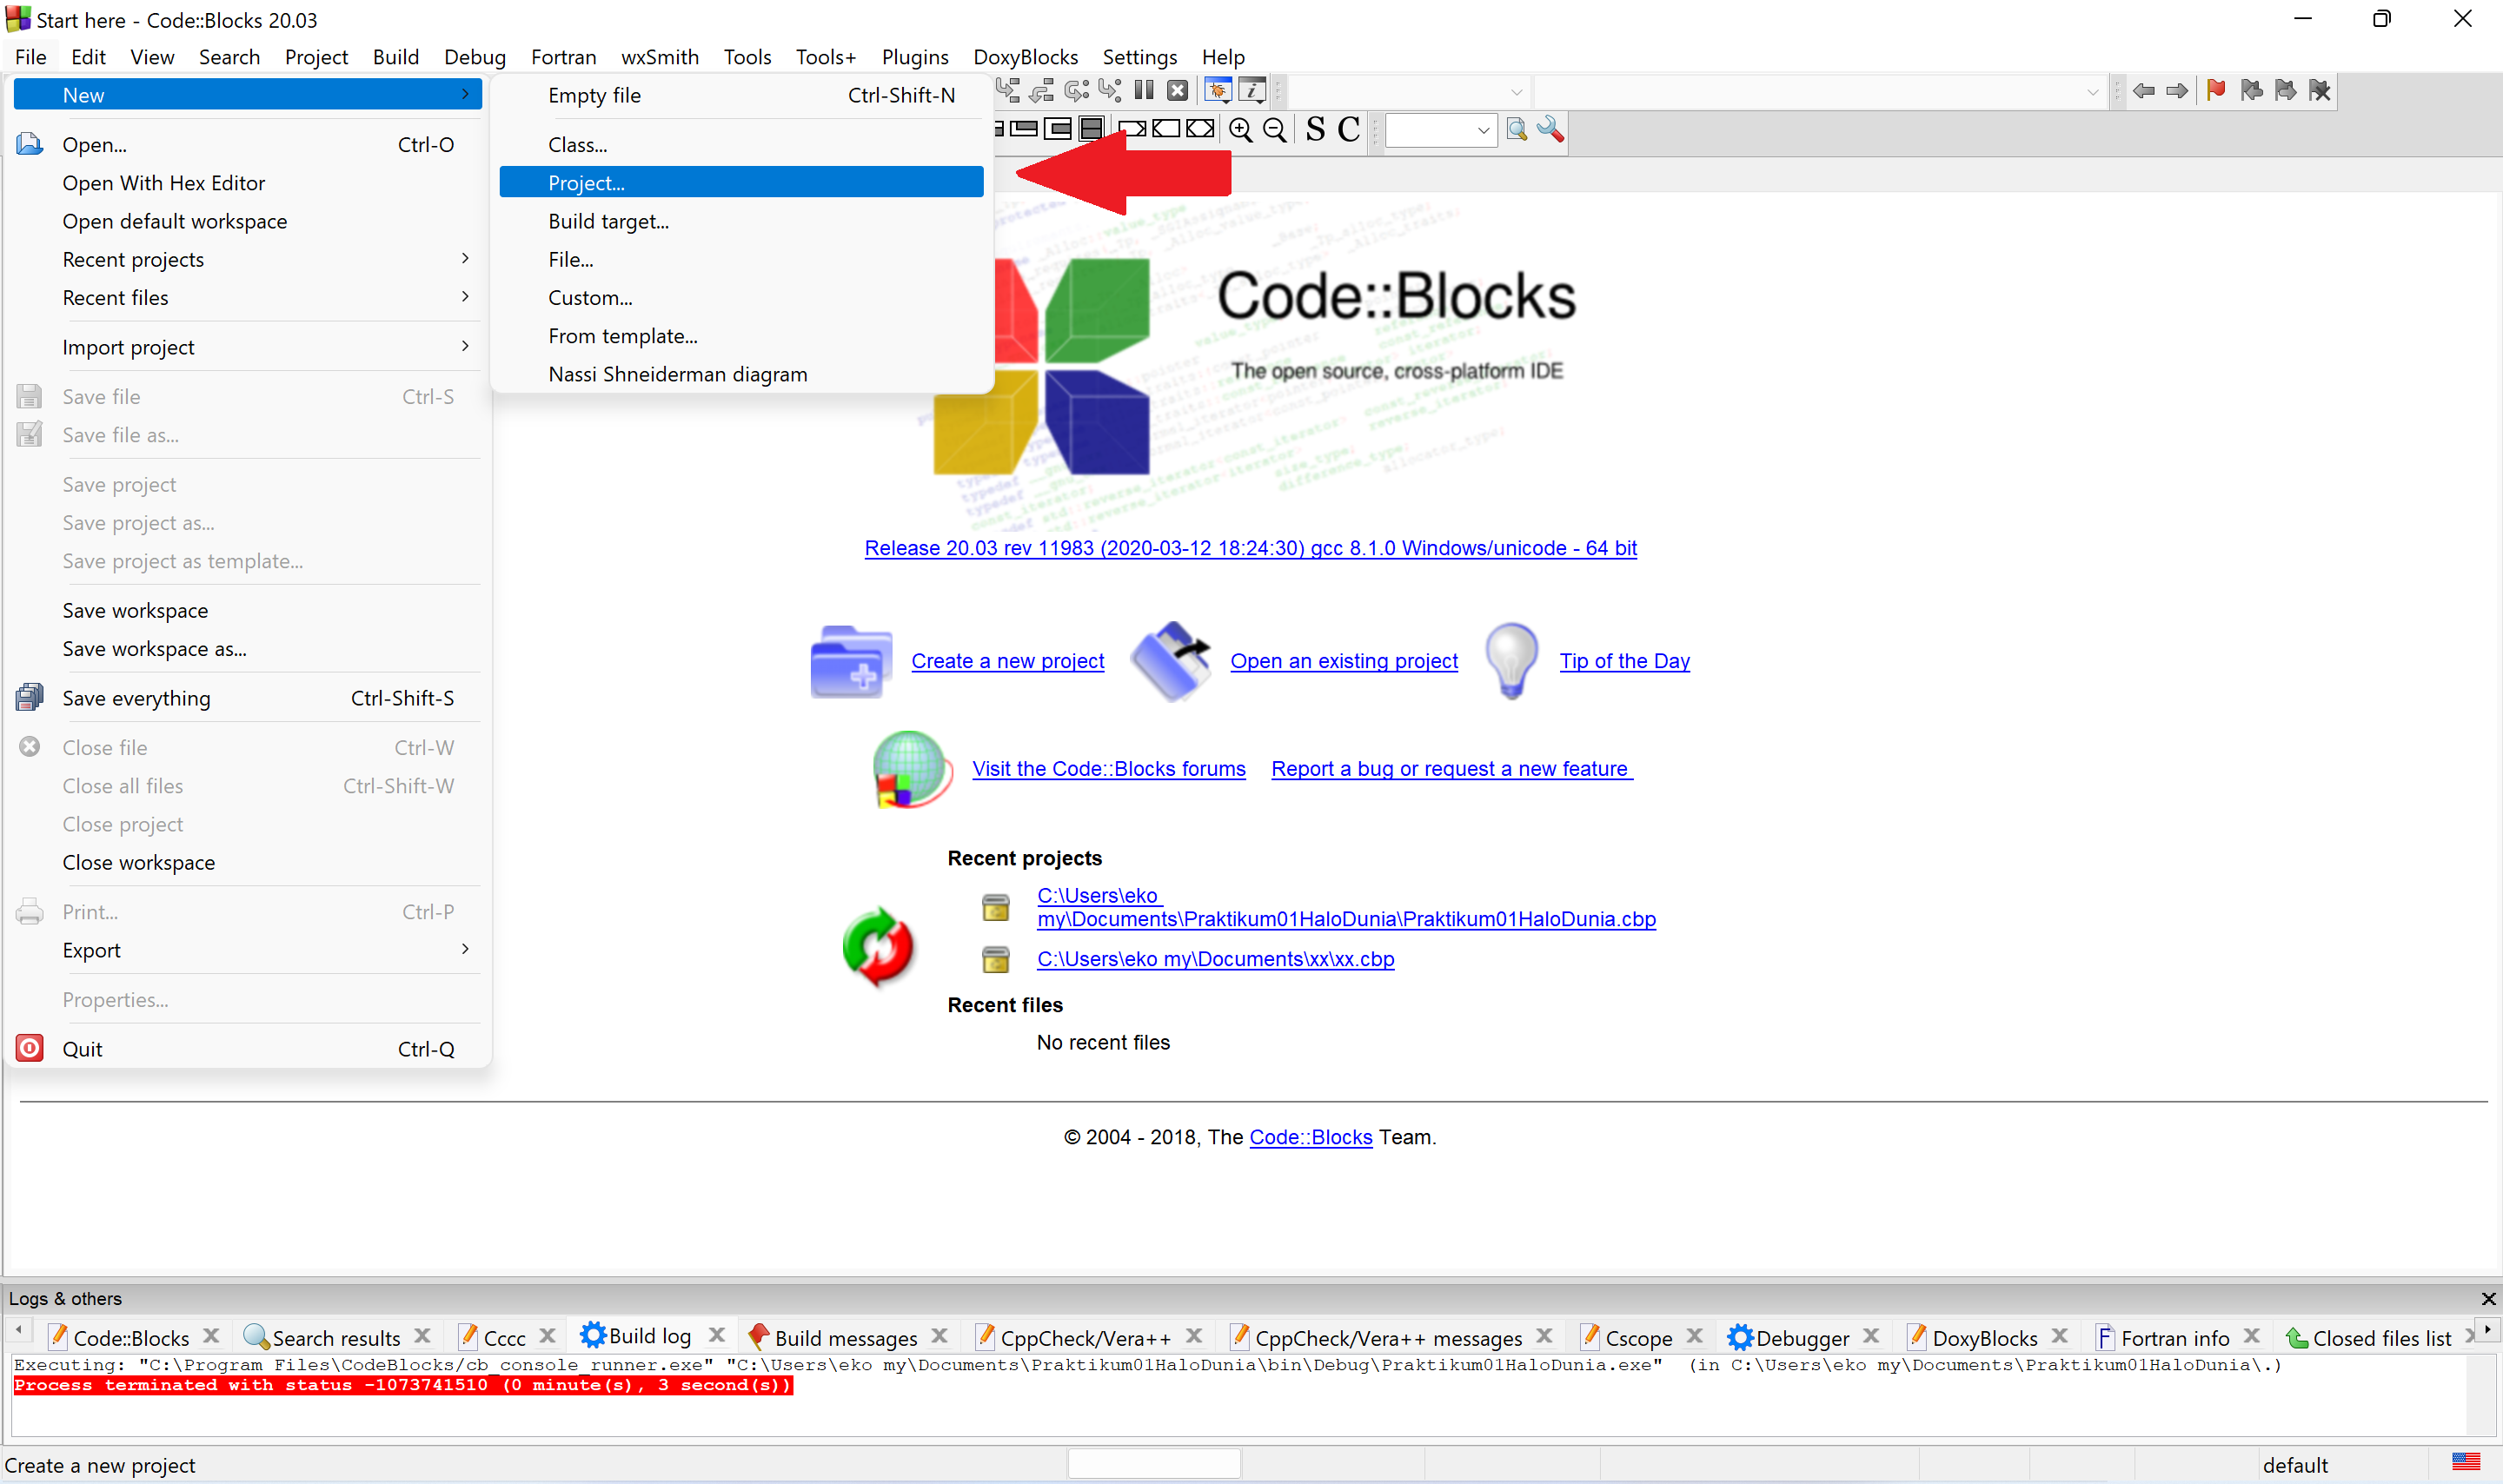
\includegraphics[width=0.7\linewidth]{P1/img/screenshot002.png}
		      \caption{}
		      \label{fig:screenshot002}
	      \end{figure}
	\item Click on Console Application
	      \begin{figure}[H]
		      \centering
		      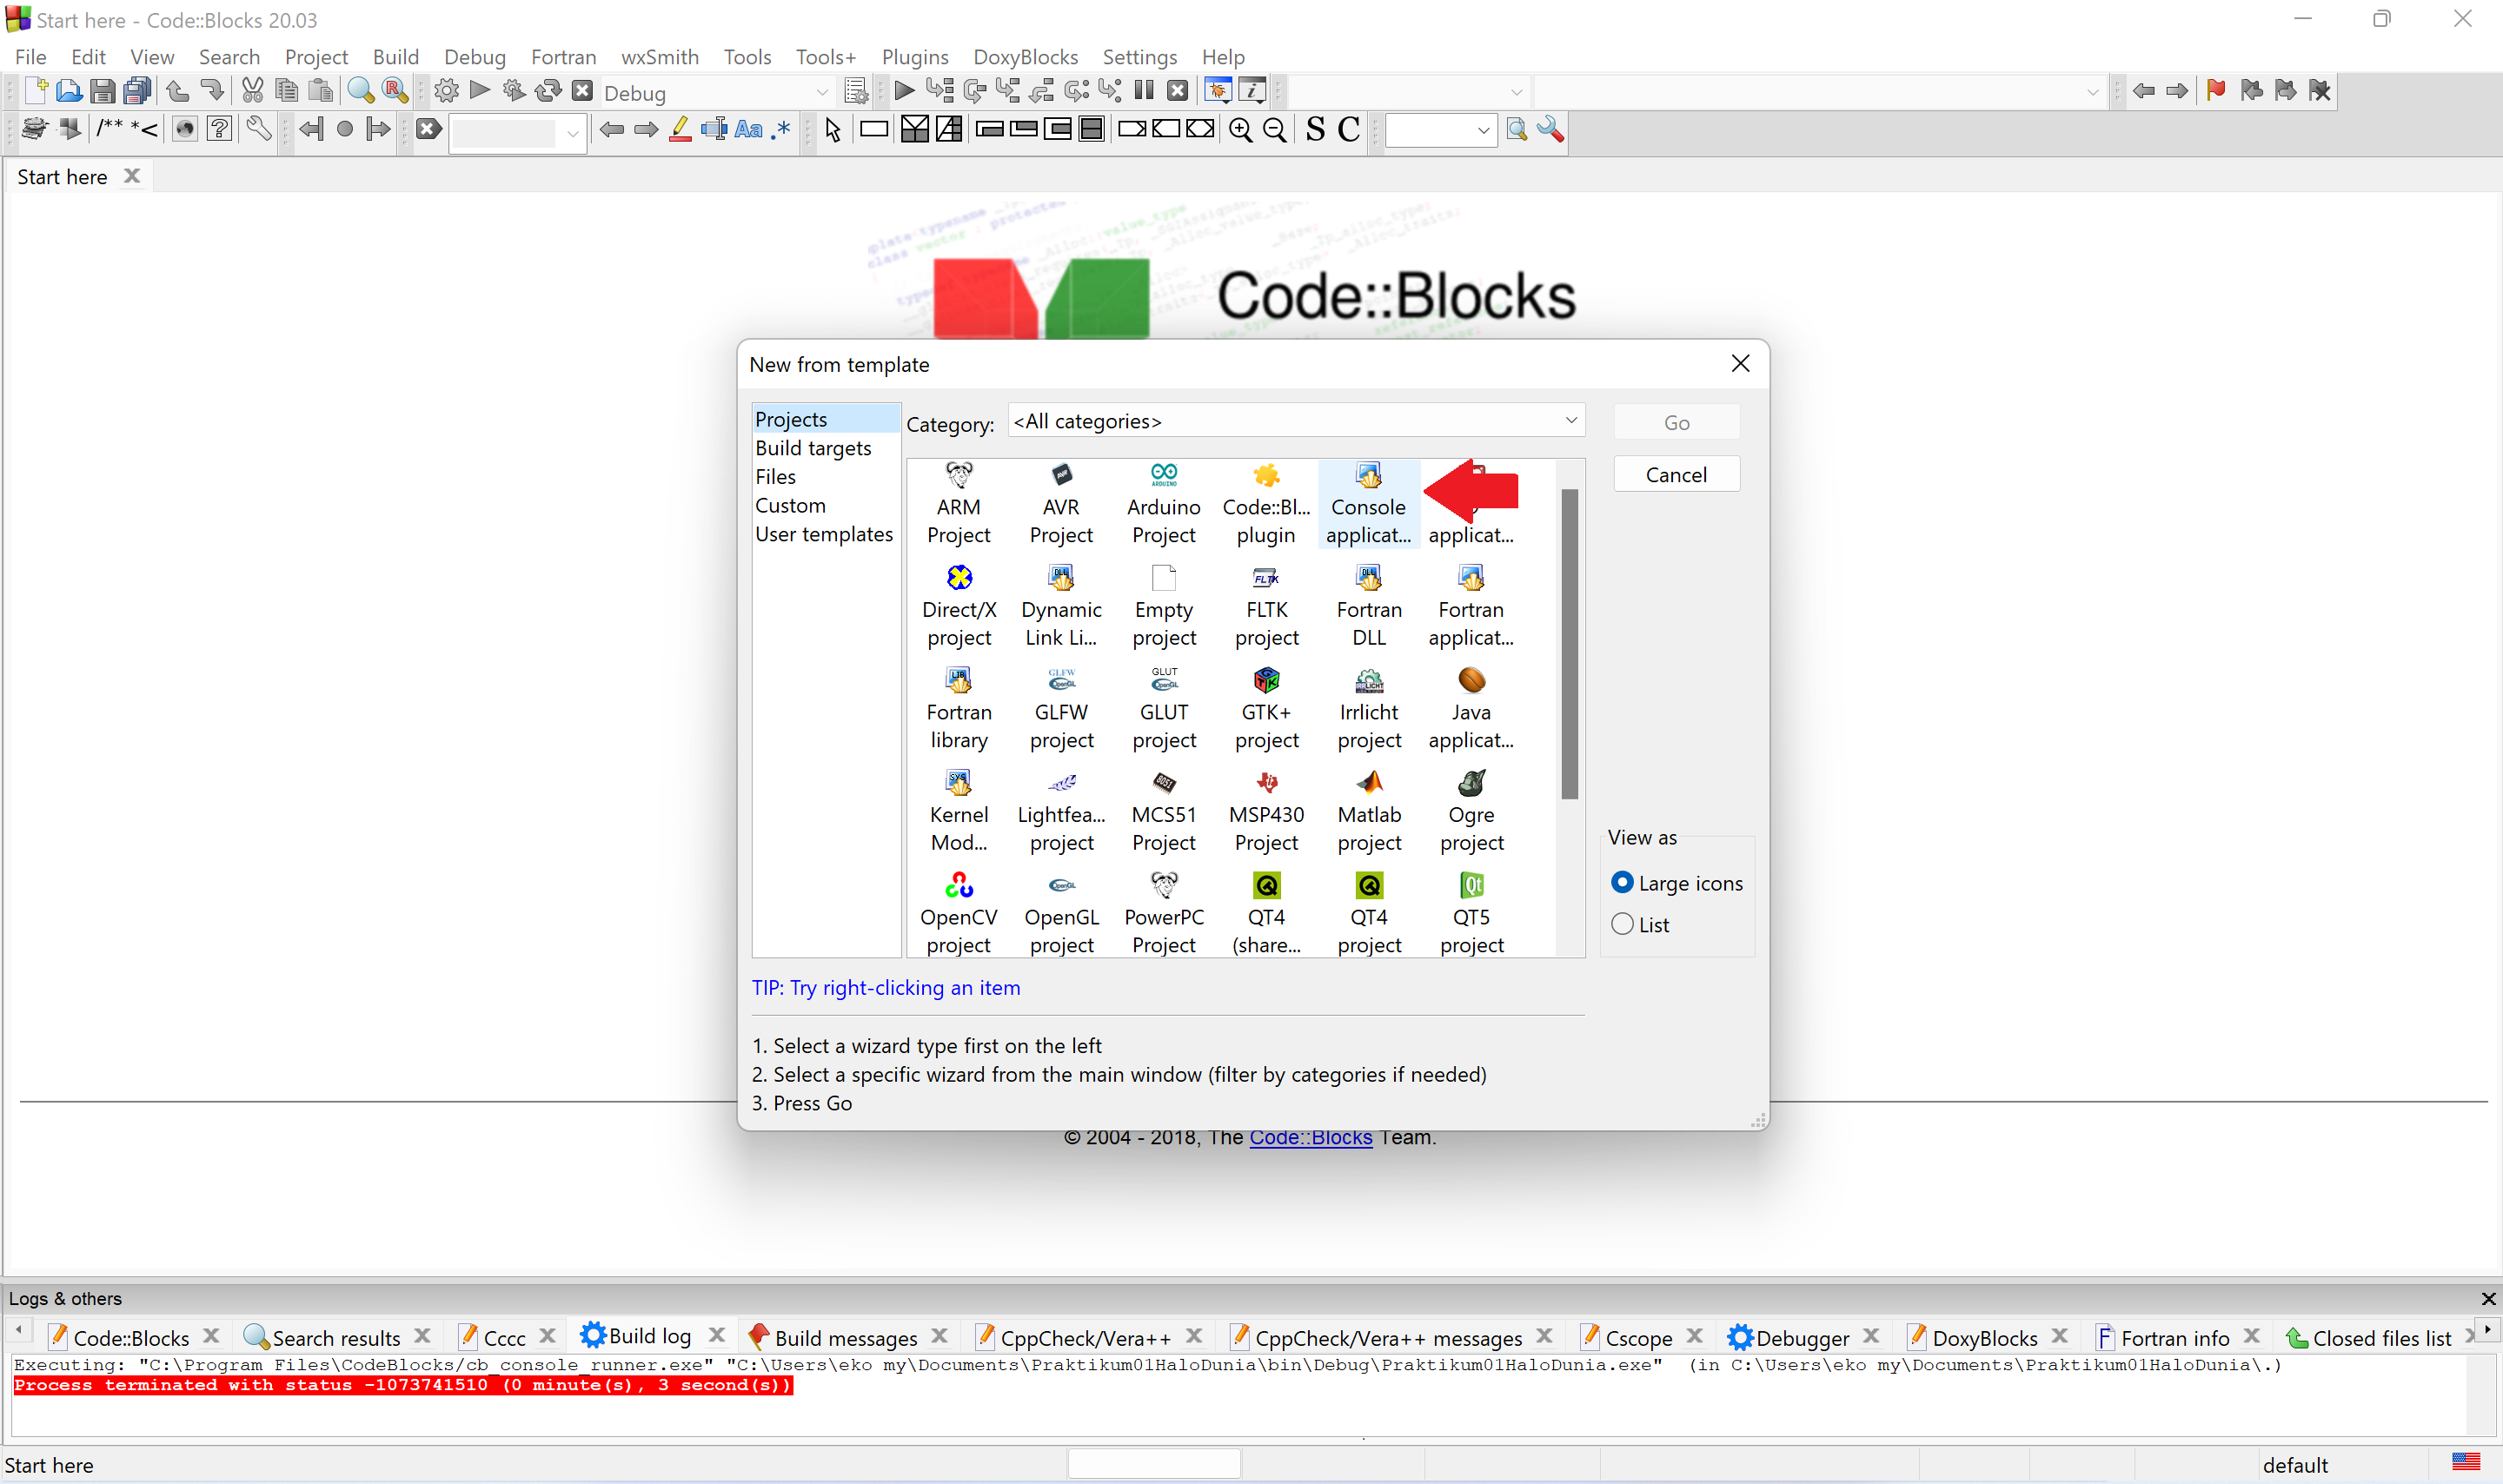
\includegraphics[width=0.7\linewidth]{P1/img/screenshot004.png}
		      \caption{}
		      \label{fig:screenshot004}
	      \end{figure}
	\item Choose C as the programming language
	      \begin{figure}[H]
		      \centering
		      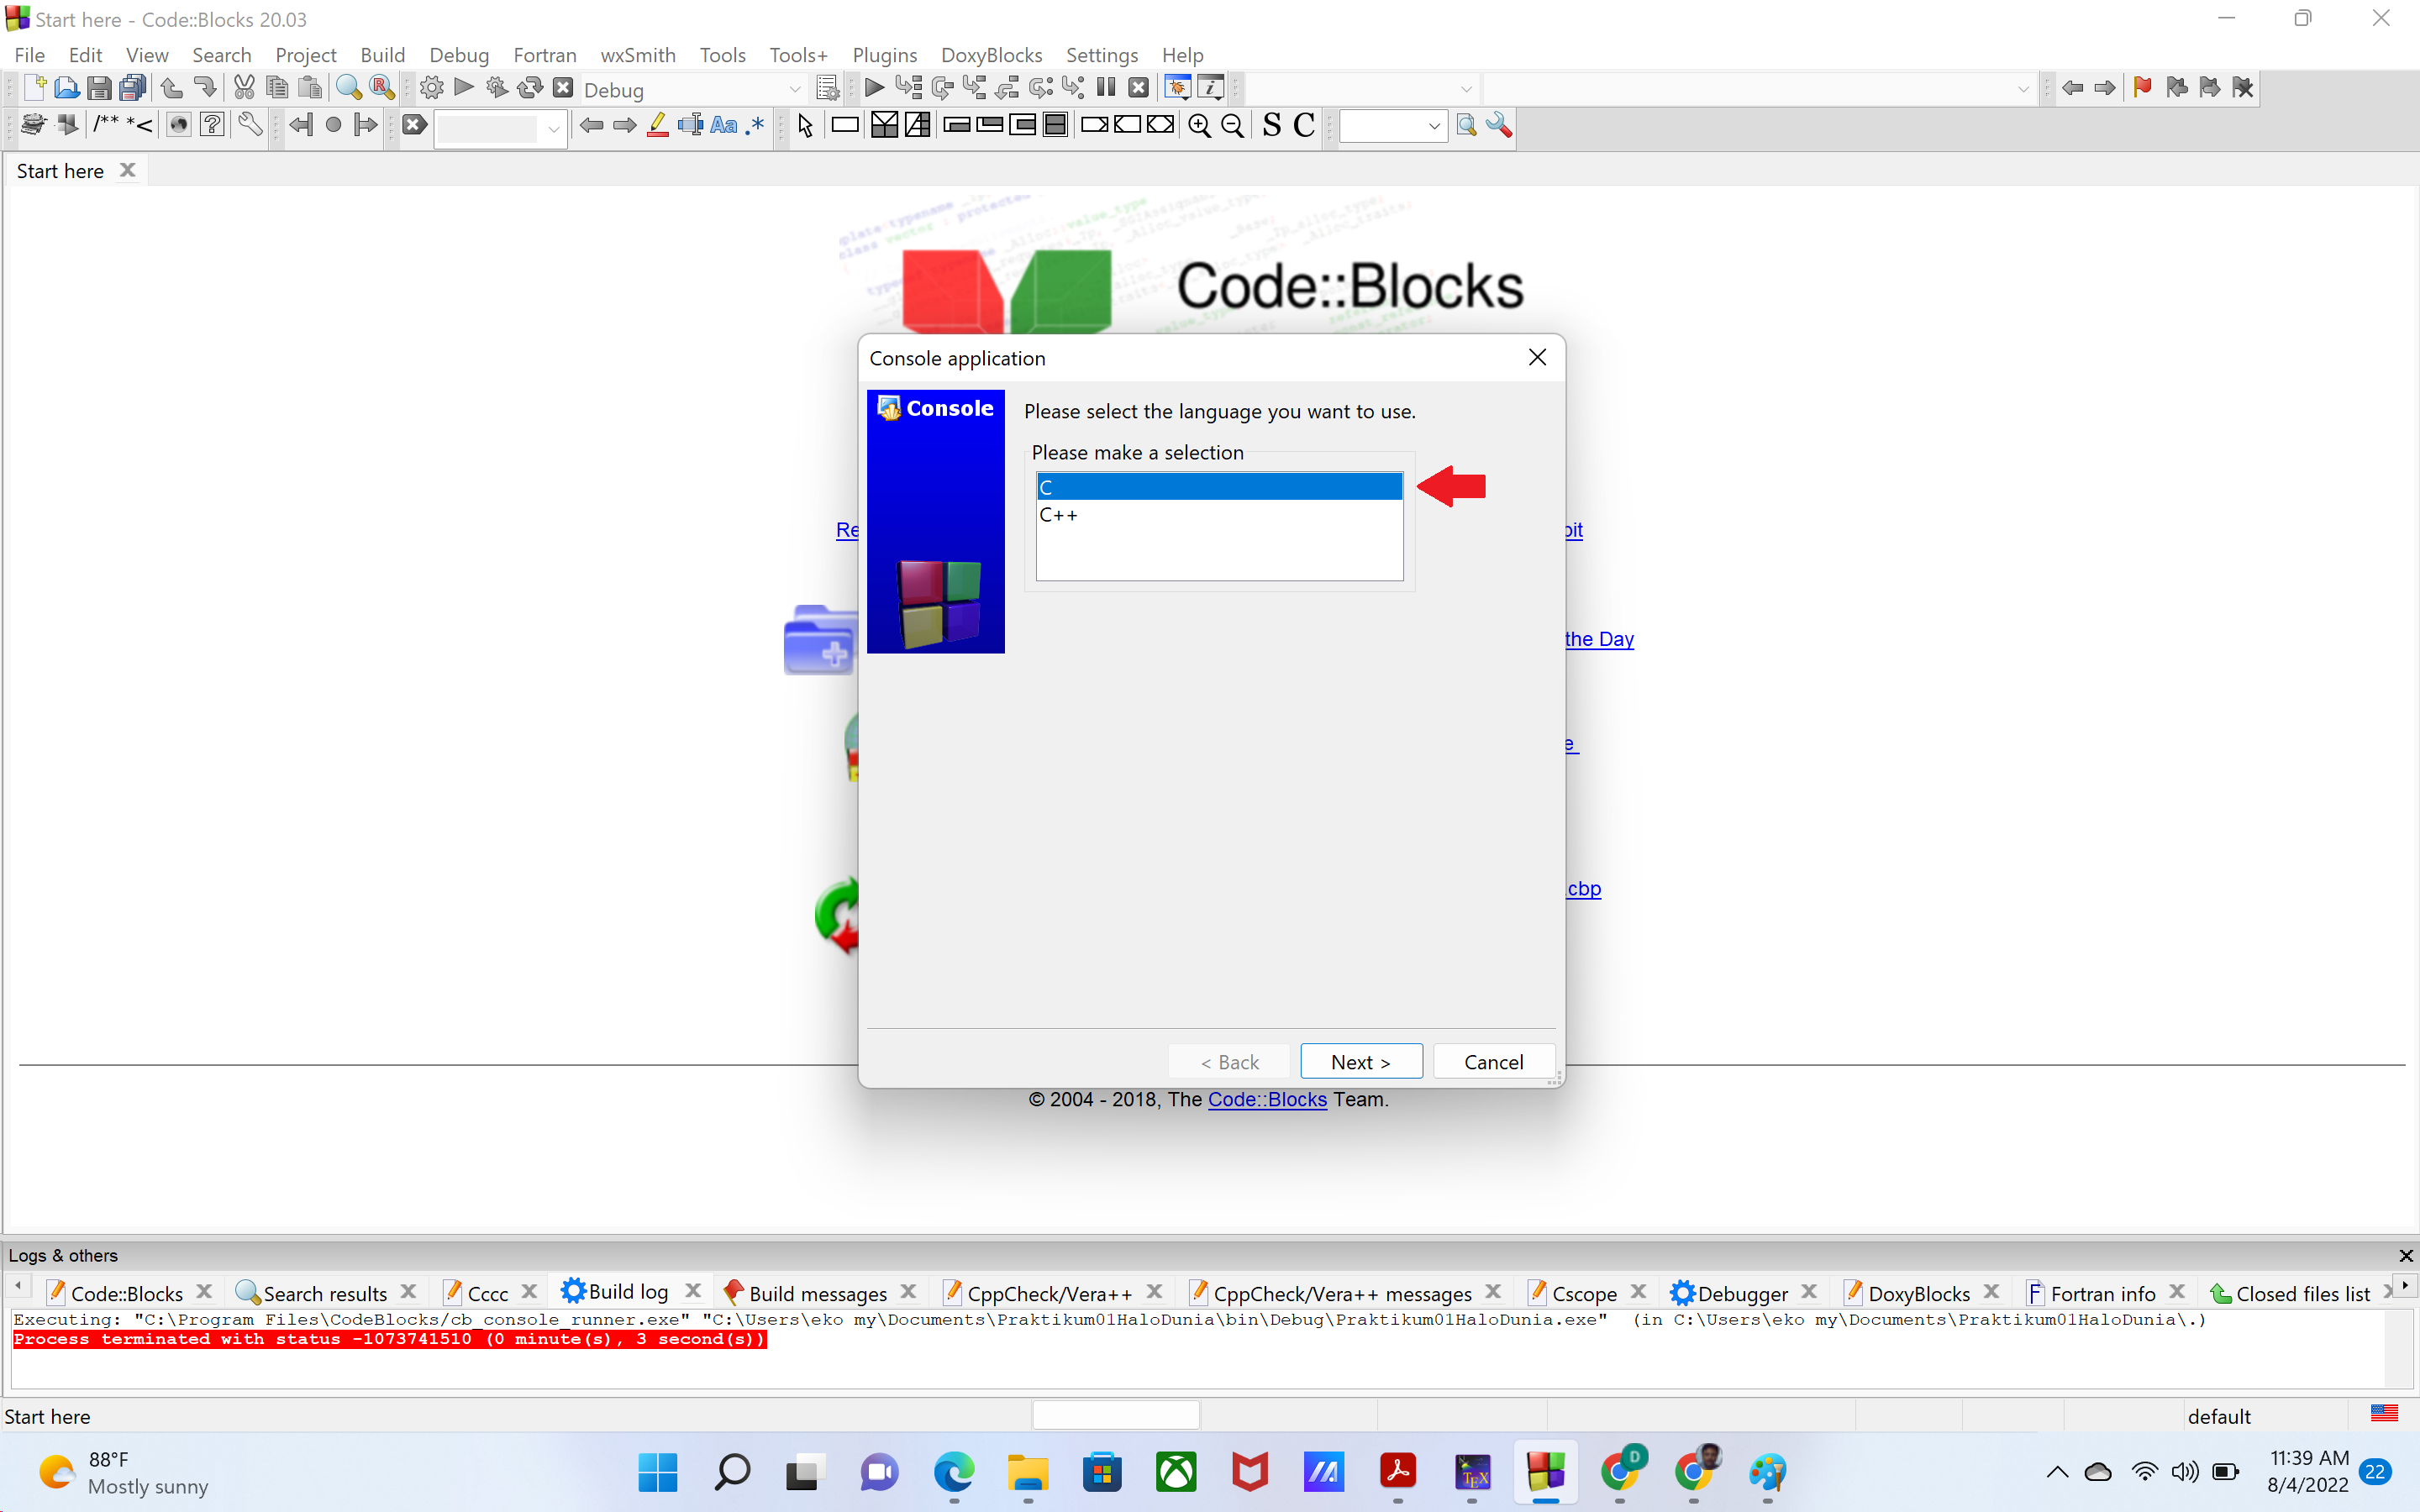
\includegraphics[width=0.7\linewidth]{P1/img/screenshot005.png}
		      \caption{}
		      \label{fig:screenshot005}
	      \end{figure}
	\item Insert your project name
	      \begin{figure}[H]
		      \centering
		      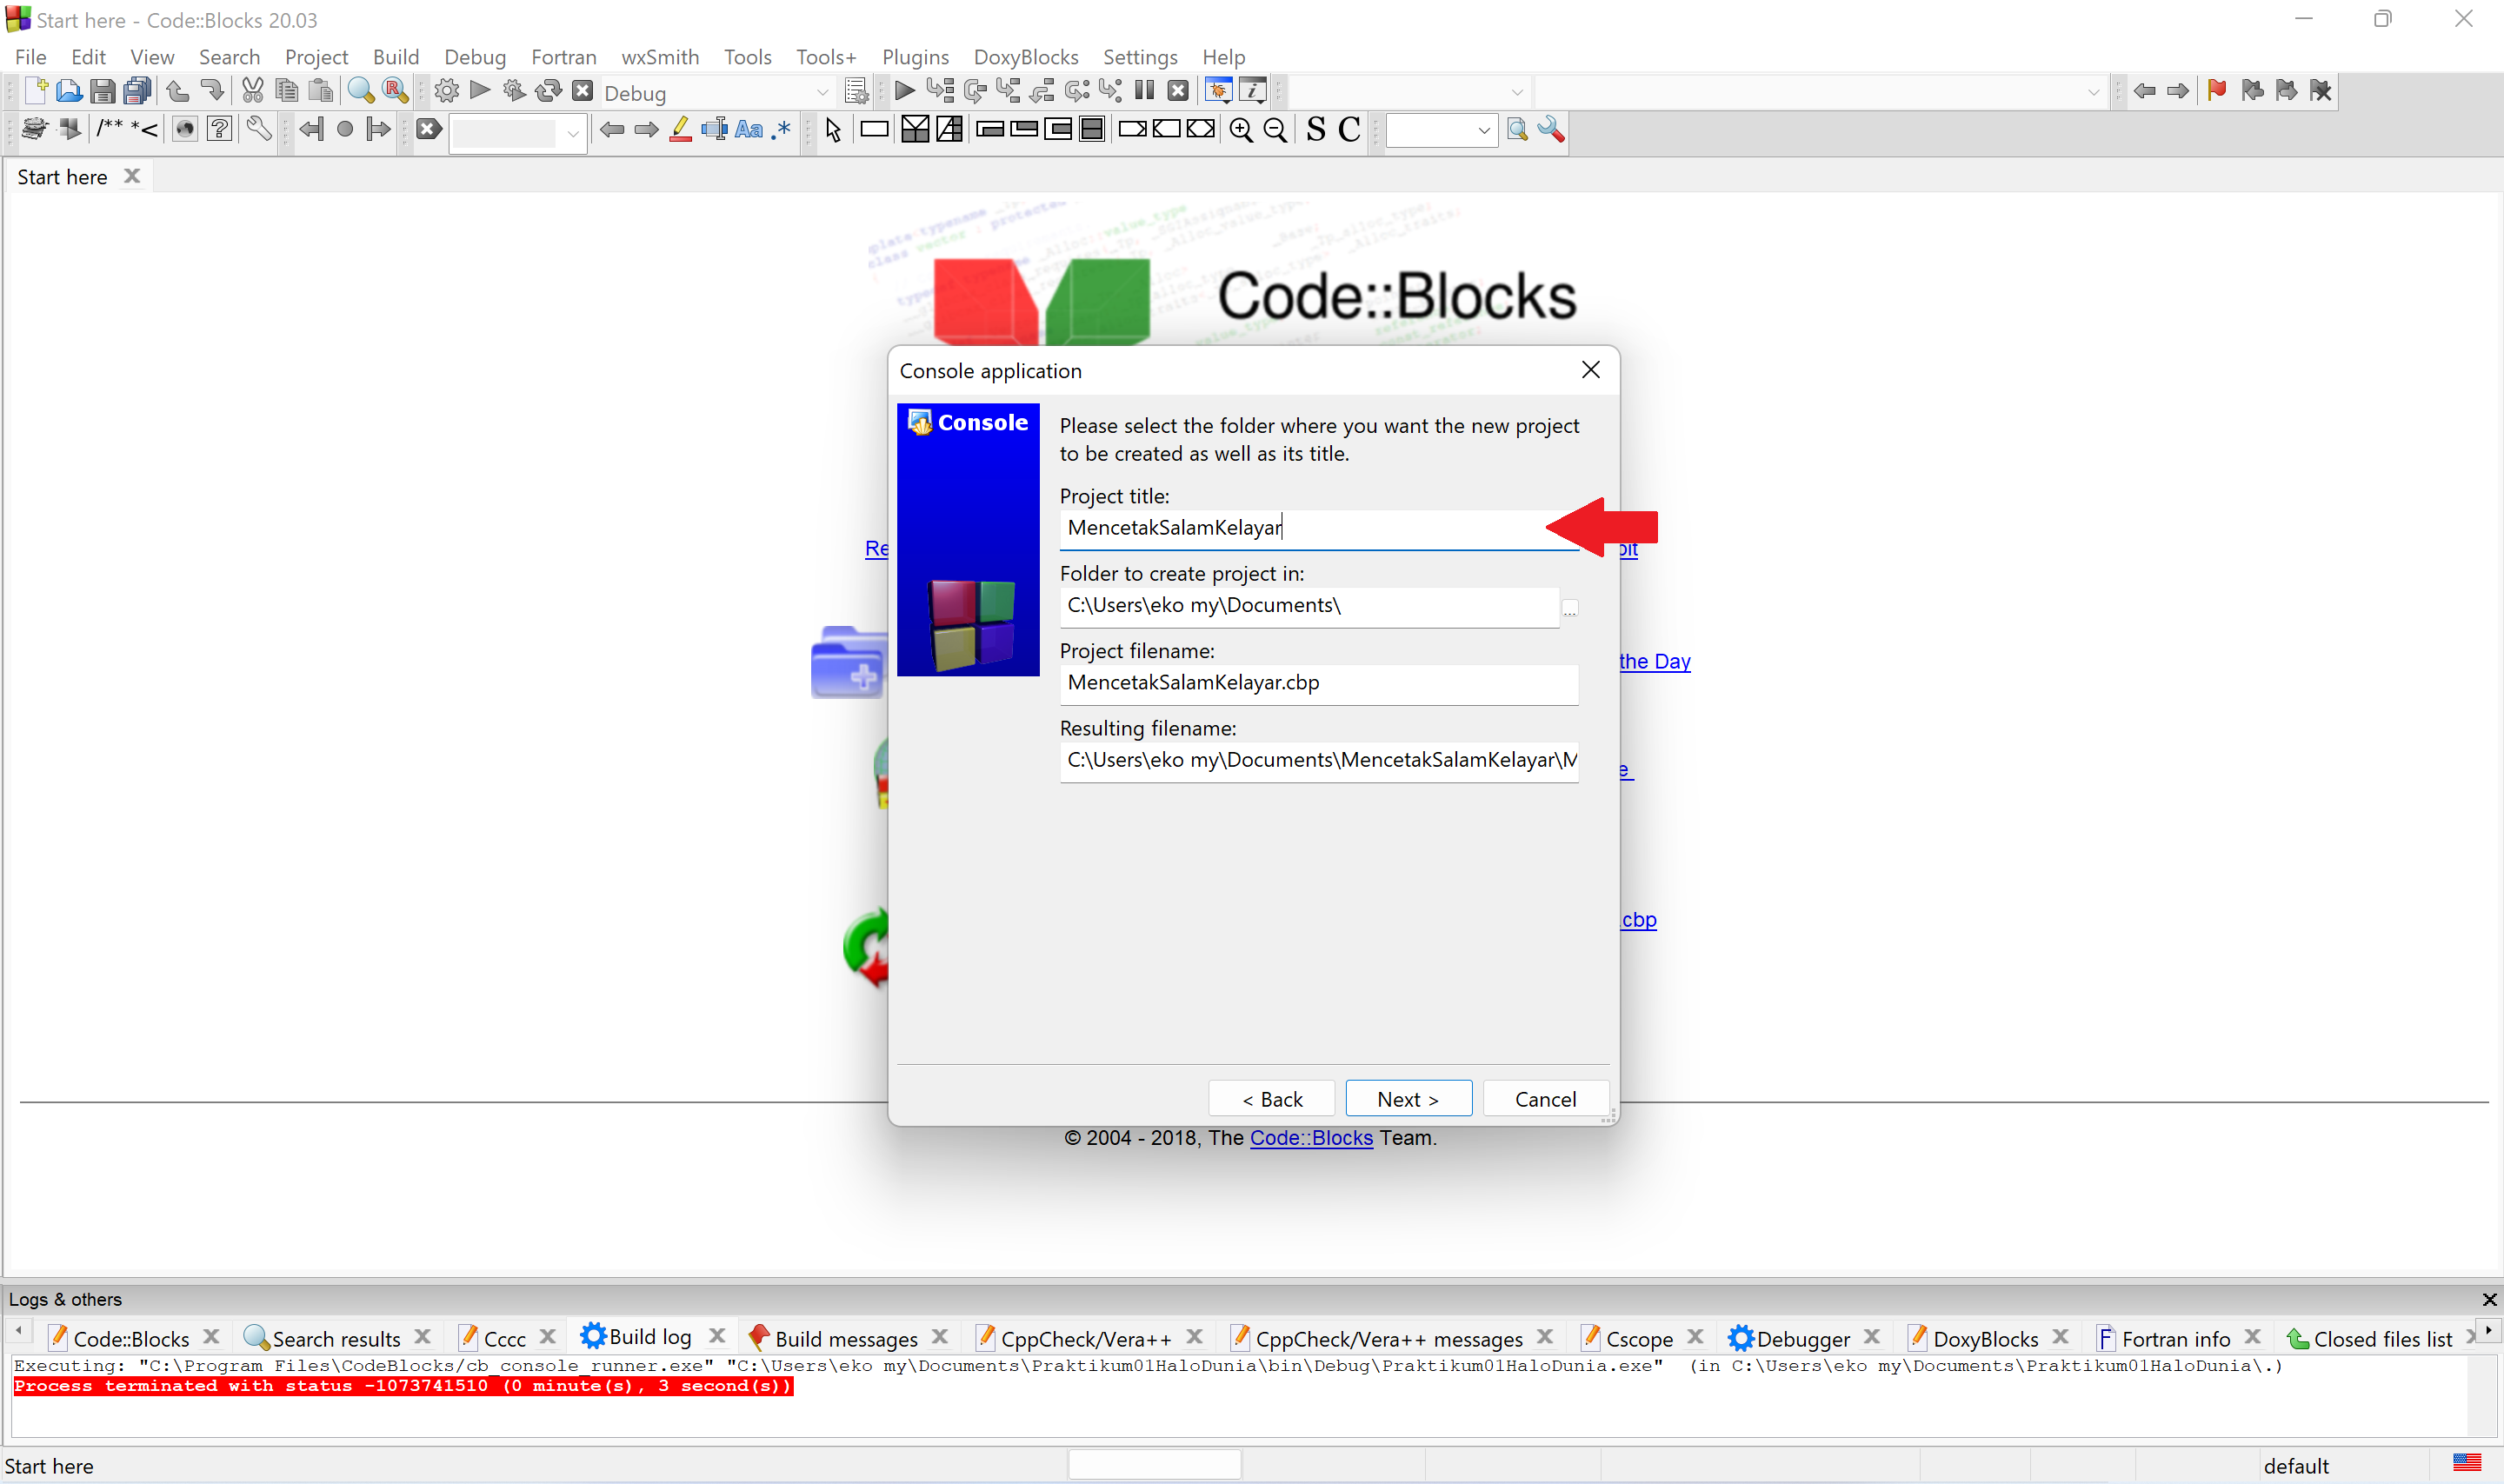
\includegraphics[width=0.7\linewidth]{P1/img/screenshot006.png}
		      \caption{}
		      \label{fig:screenshot006}
	      \end{figure}
	\item Choose the compiler (gcc), select a directory to save your project, and click save
	      \begin{figure}[H]
		      \centering
		      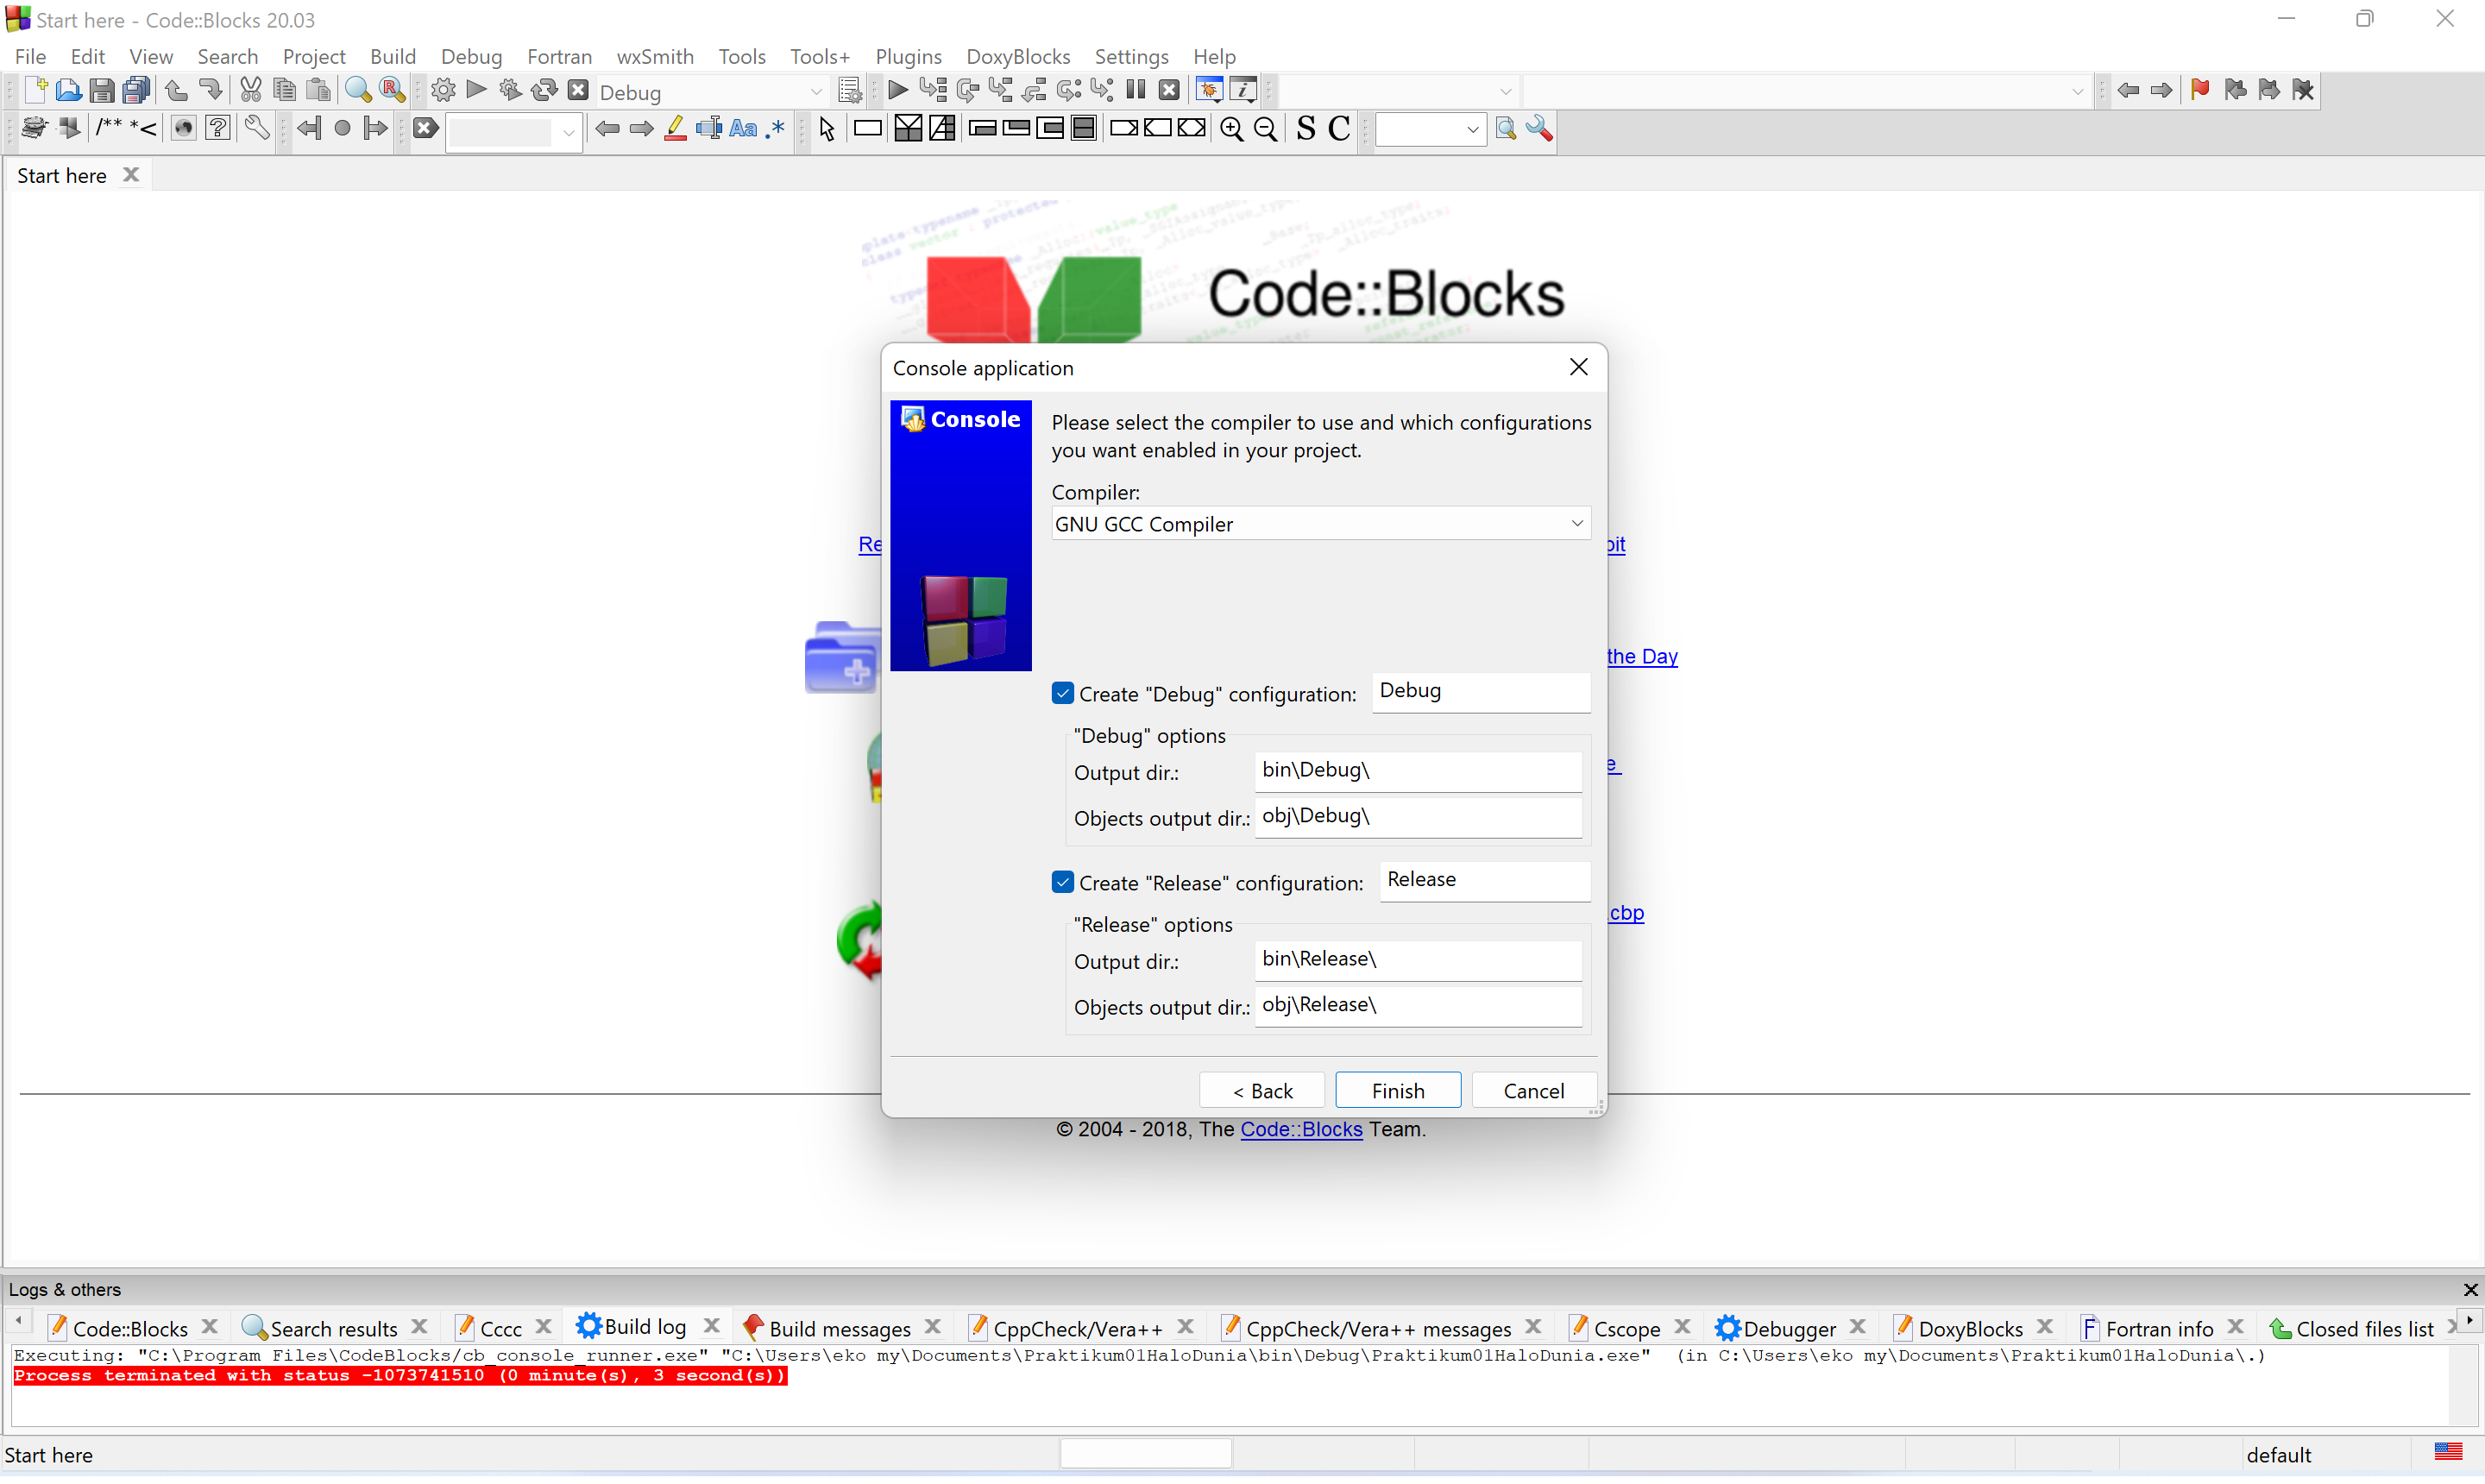
\includegraphics[width=0.7\linewidth]{P1/img/screenshot007.png}
		      \caption{}
		      \label{fig:screenshot007}
	      \end{figure}
	\item Write your code \ref{fig:screenshot008} in Code::Blocks
	      \begin{figure}[H]
		      \centering
		      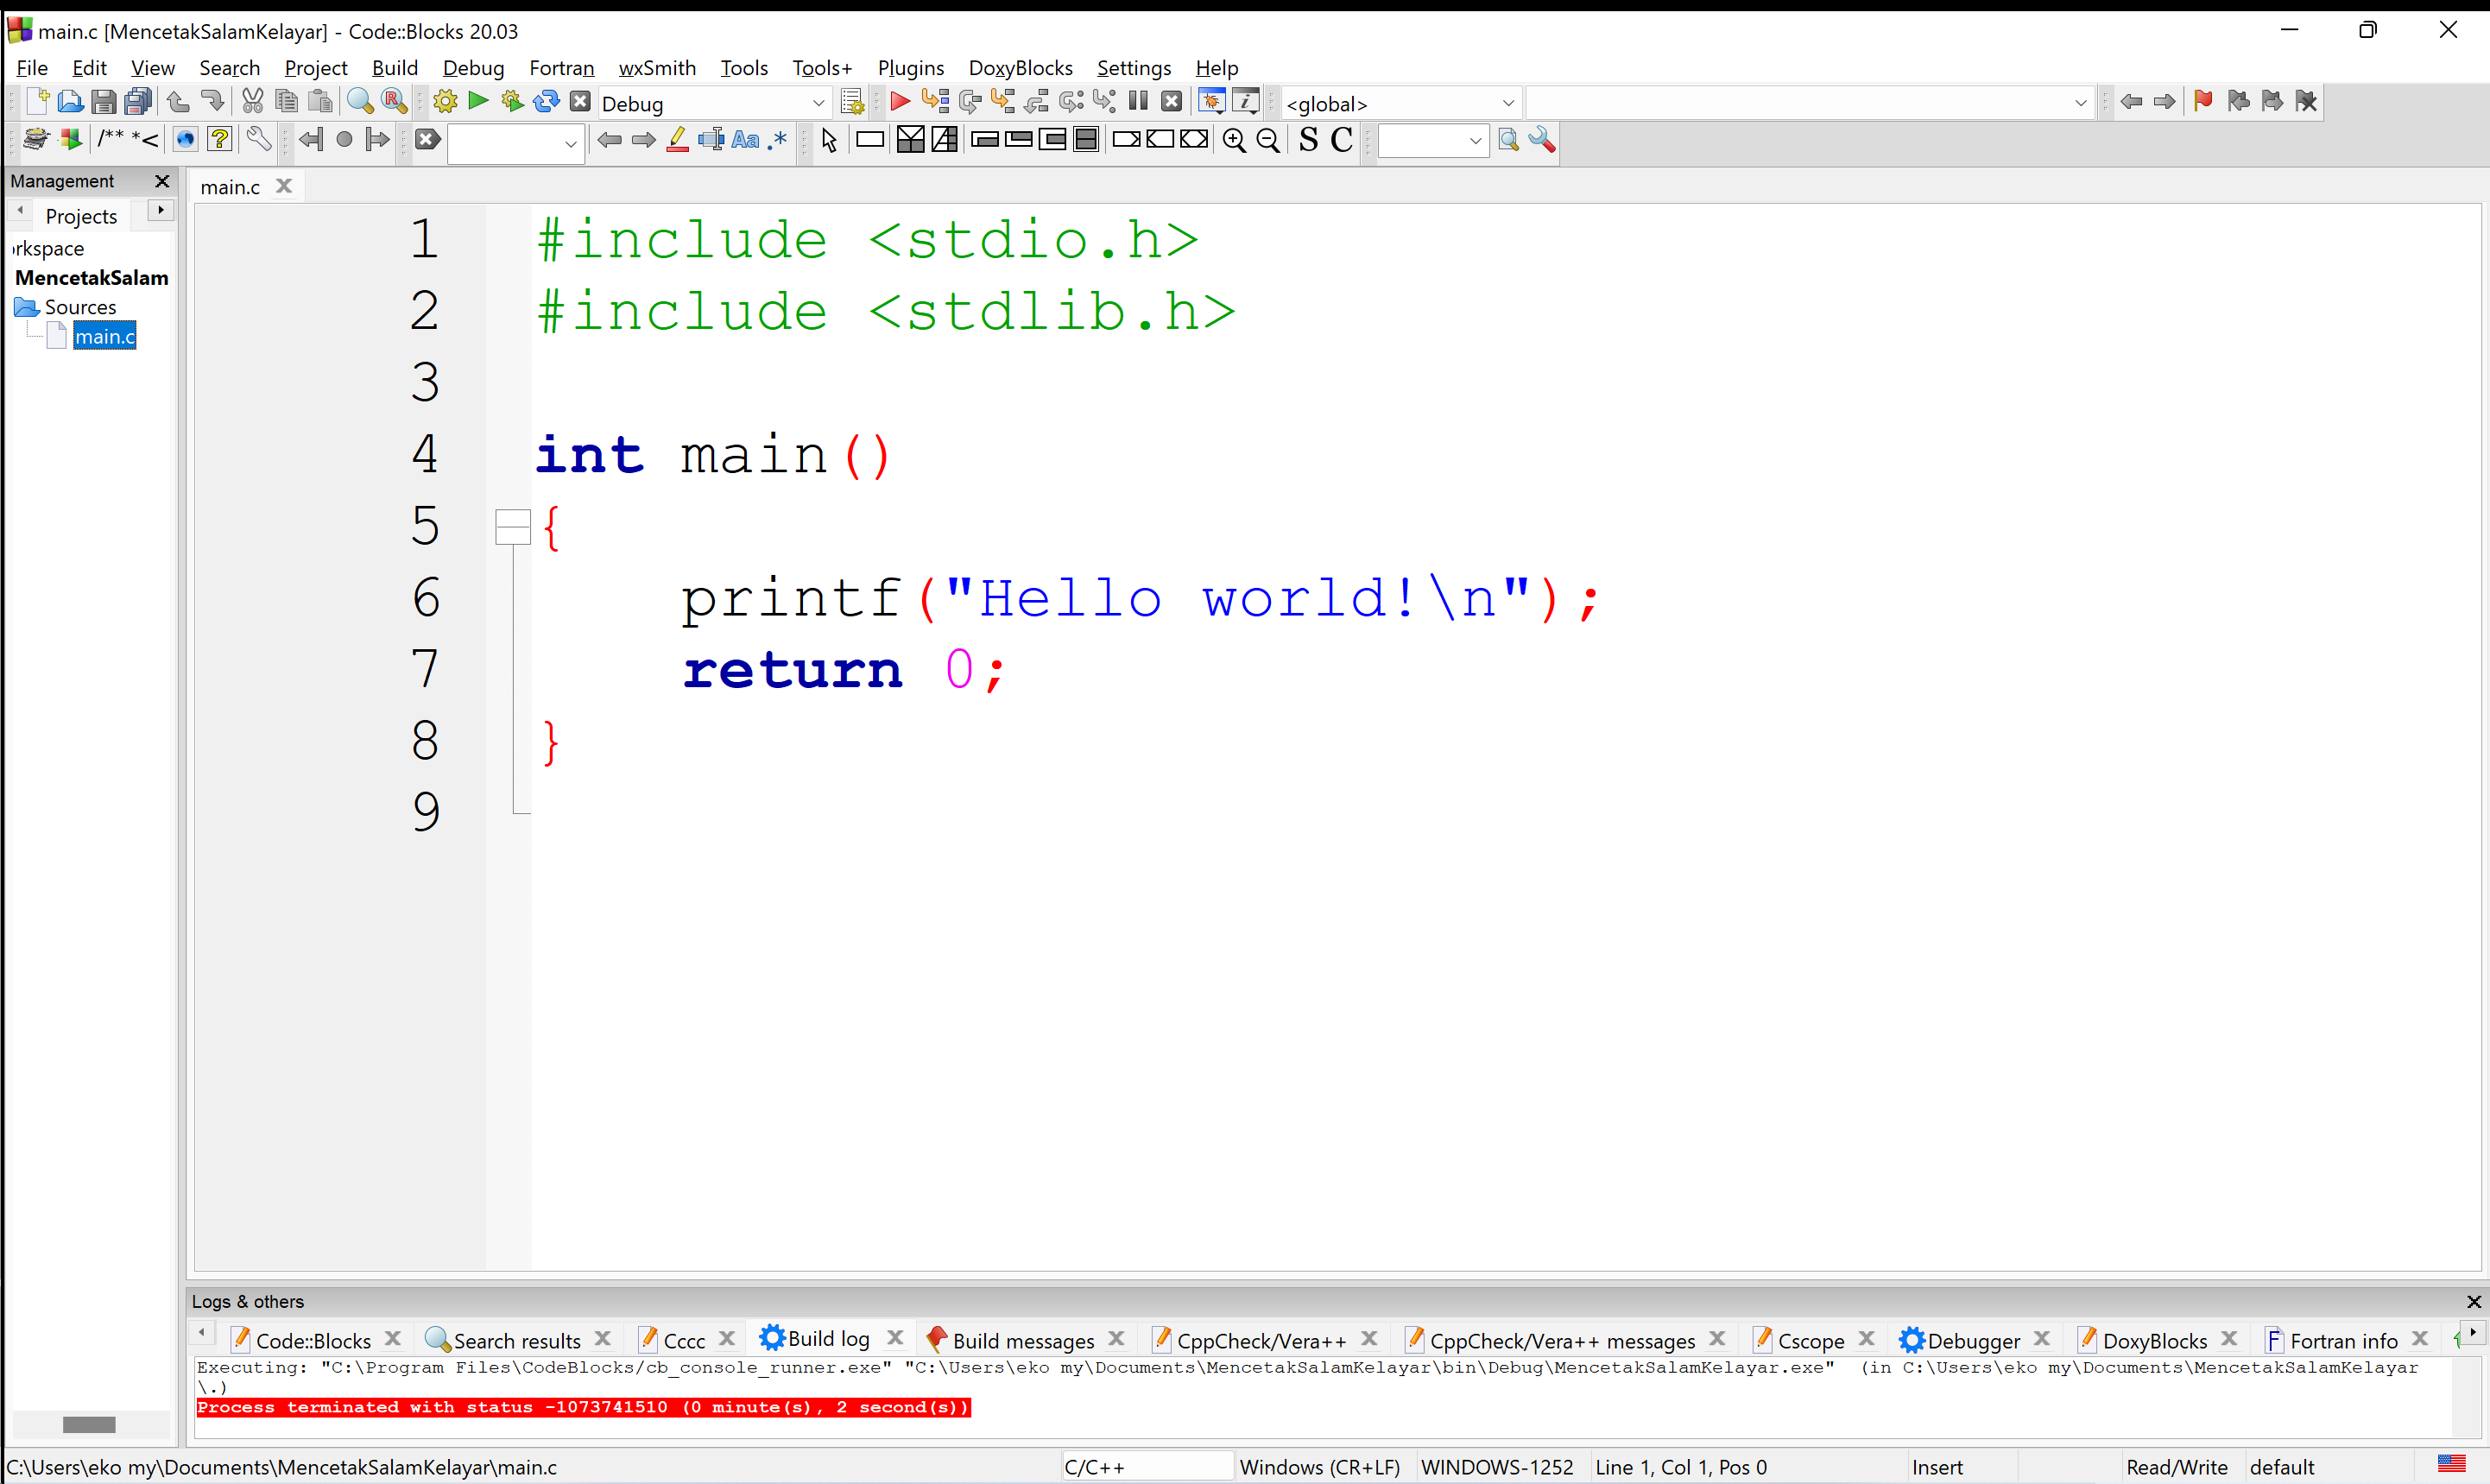
\includegraphics[width=0.7\linewidth]{P1/img/screenshot008.png}
		      \caption{}
		      \label{fig:screenshot008}
	      \end{figure}
	\item Click Build$->$Build and Run or press F9 on your keyboard
	      \begin{figure}[H]
		      \centering
		      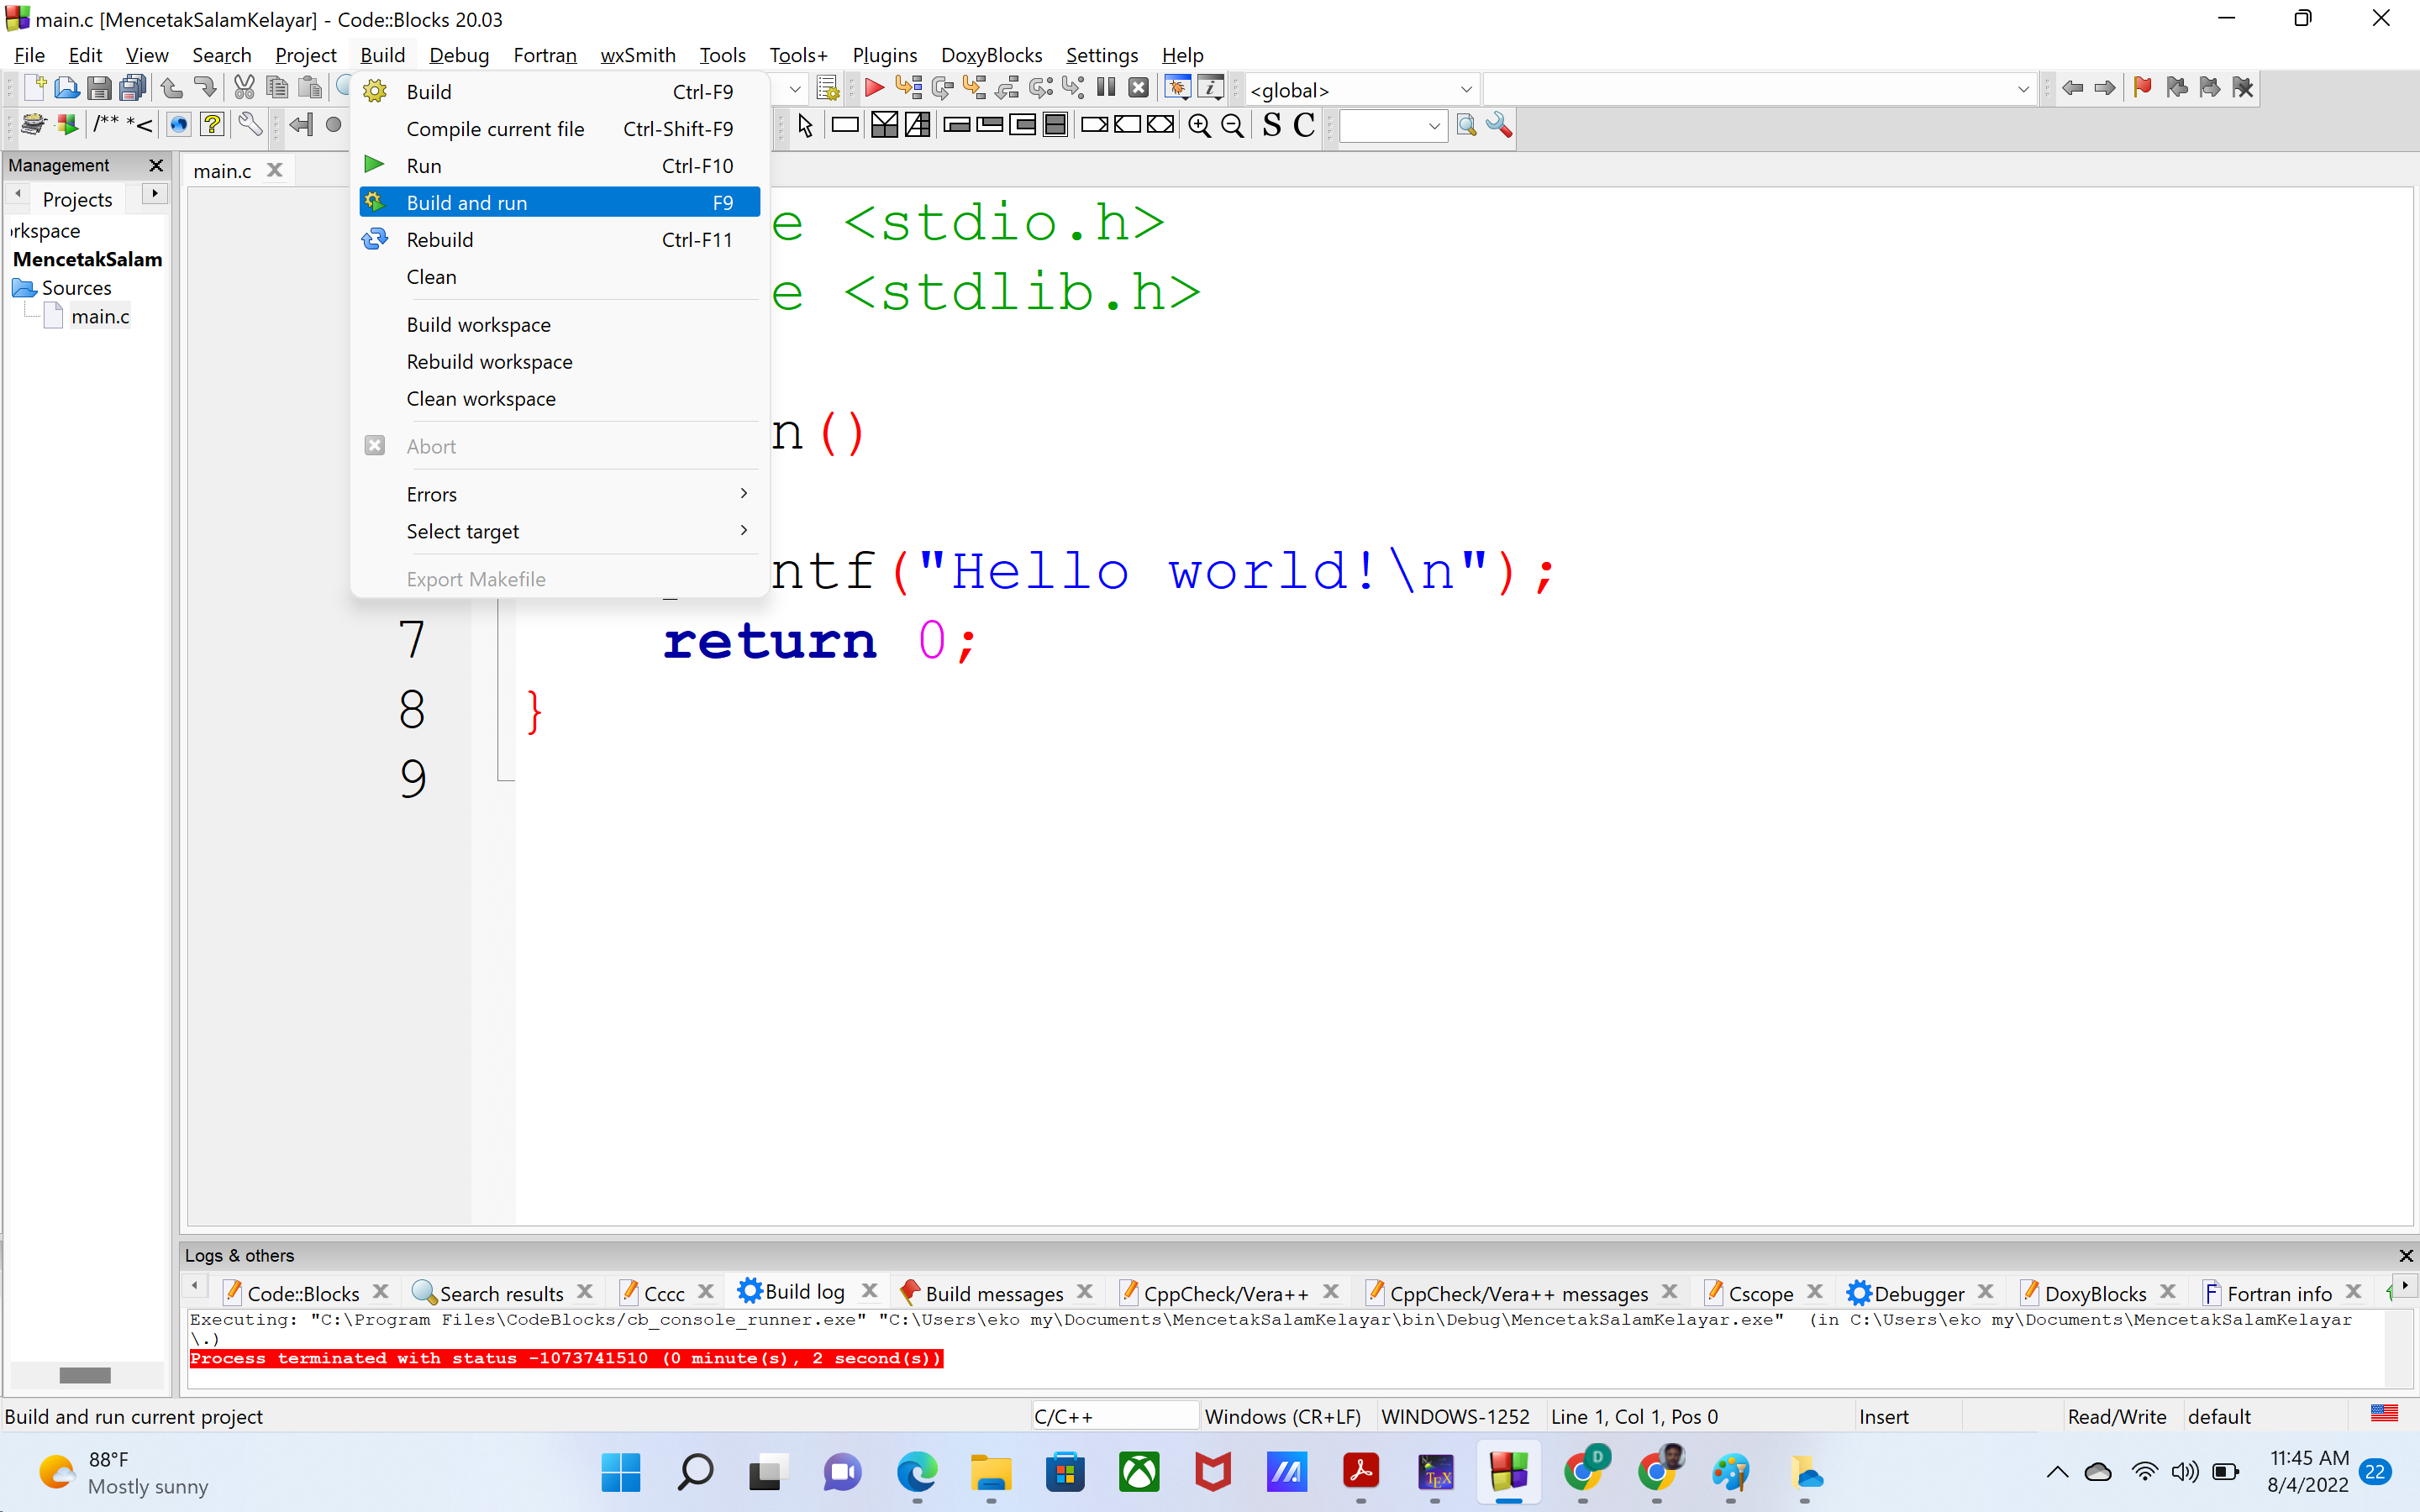
\includegraphics[width=0.7\linewidth]{P1/img/screenshot009.png}
		      \caption{}
		      \label{fig:screenshot009}
	      \end{figure}
	      % \item The program outputs can be seen on the console.
	\item The program output can be seen on the console tab
	      \begin{figure}[H]
		      \centering
		      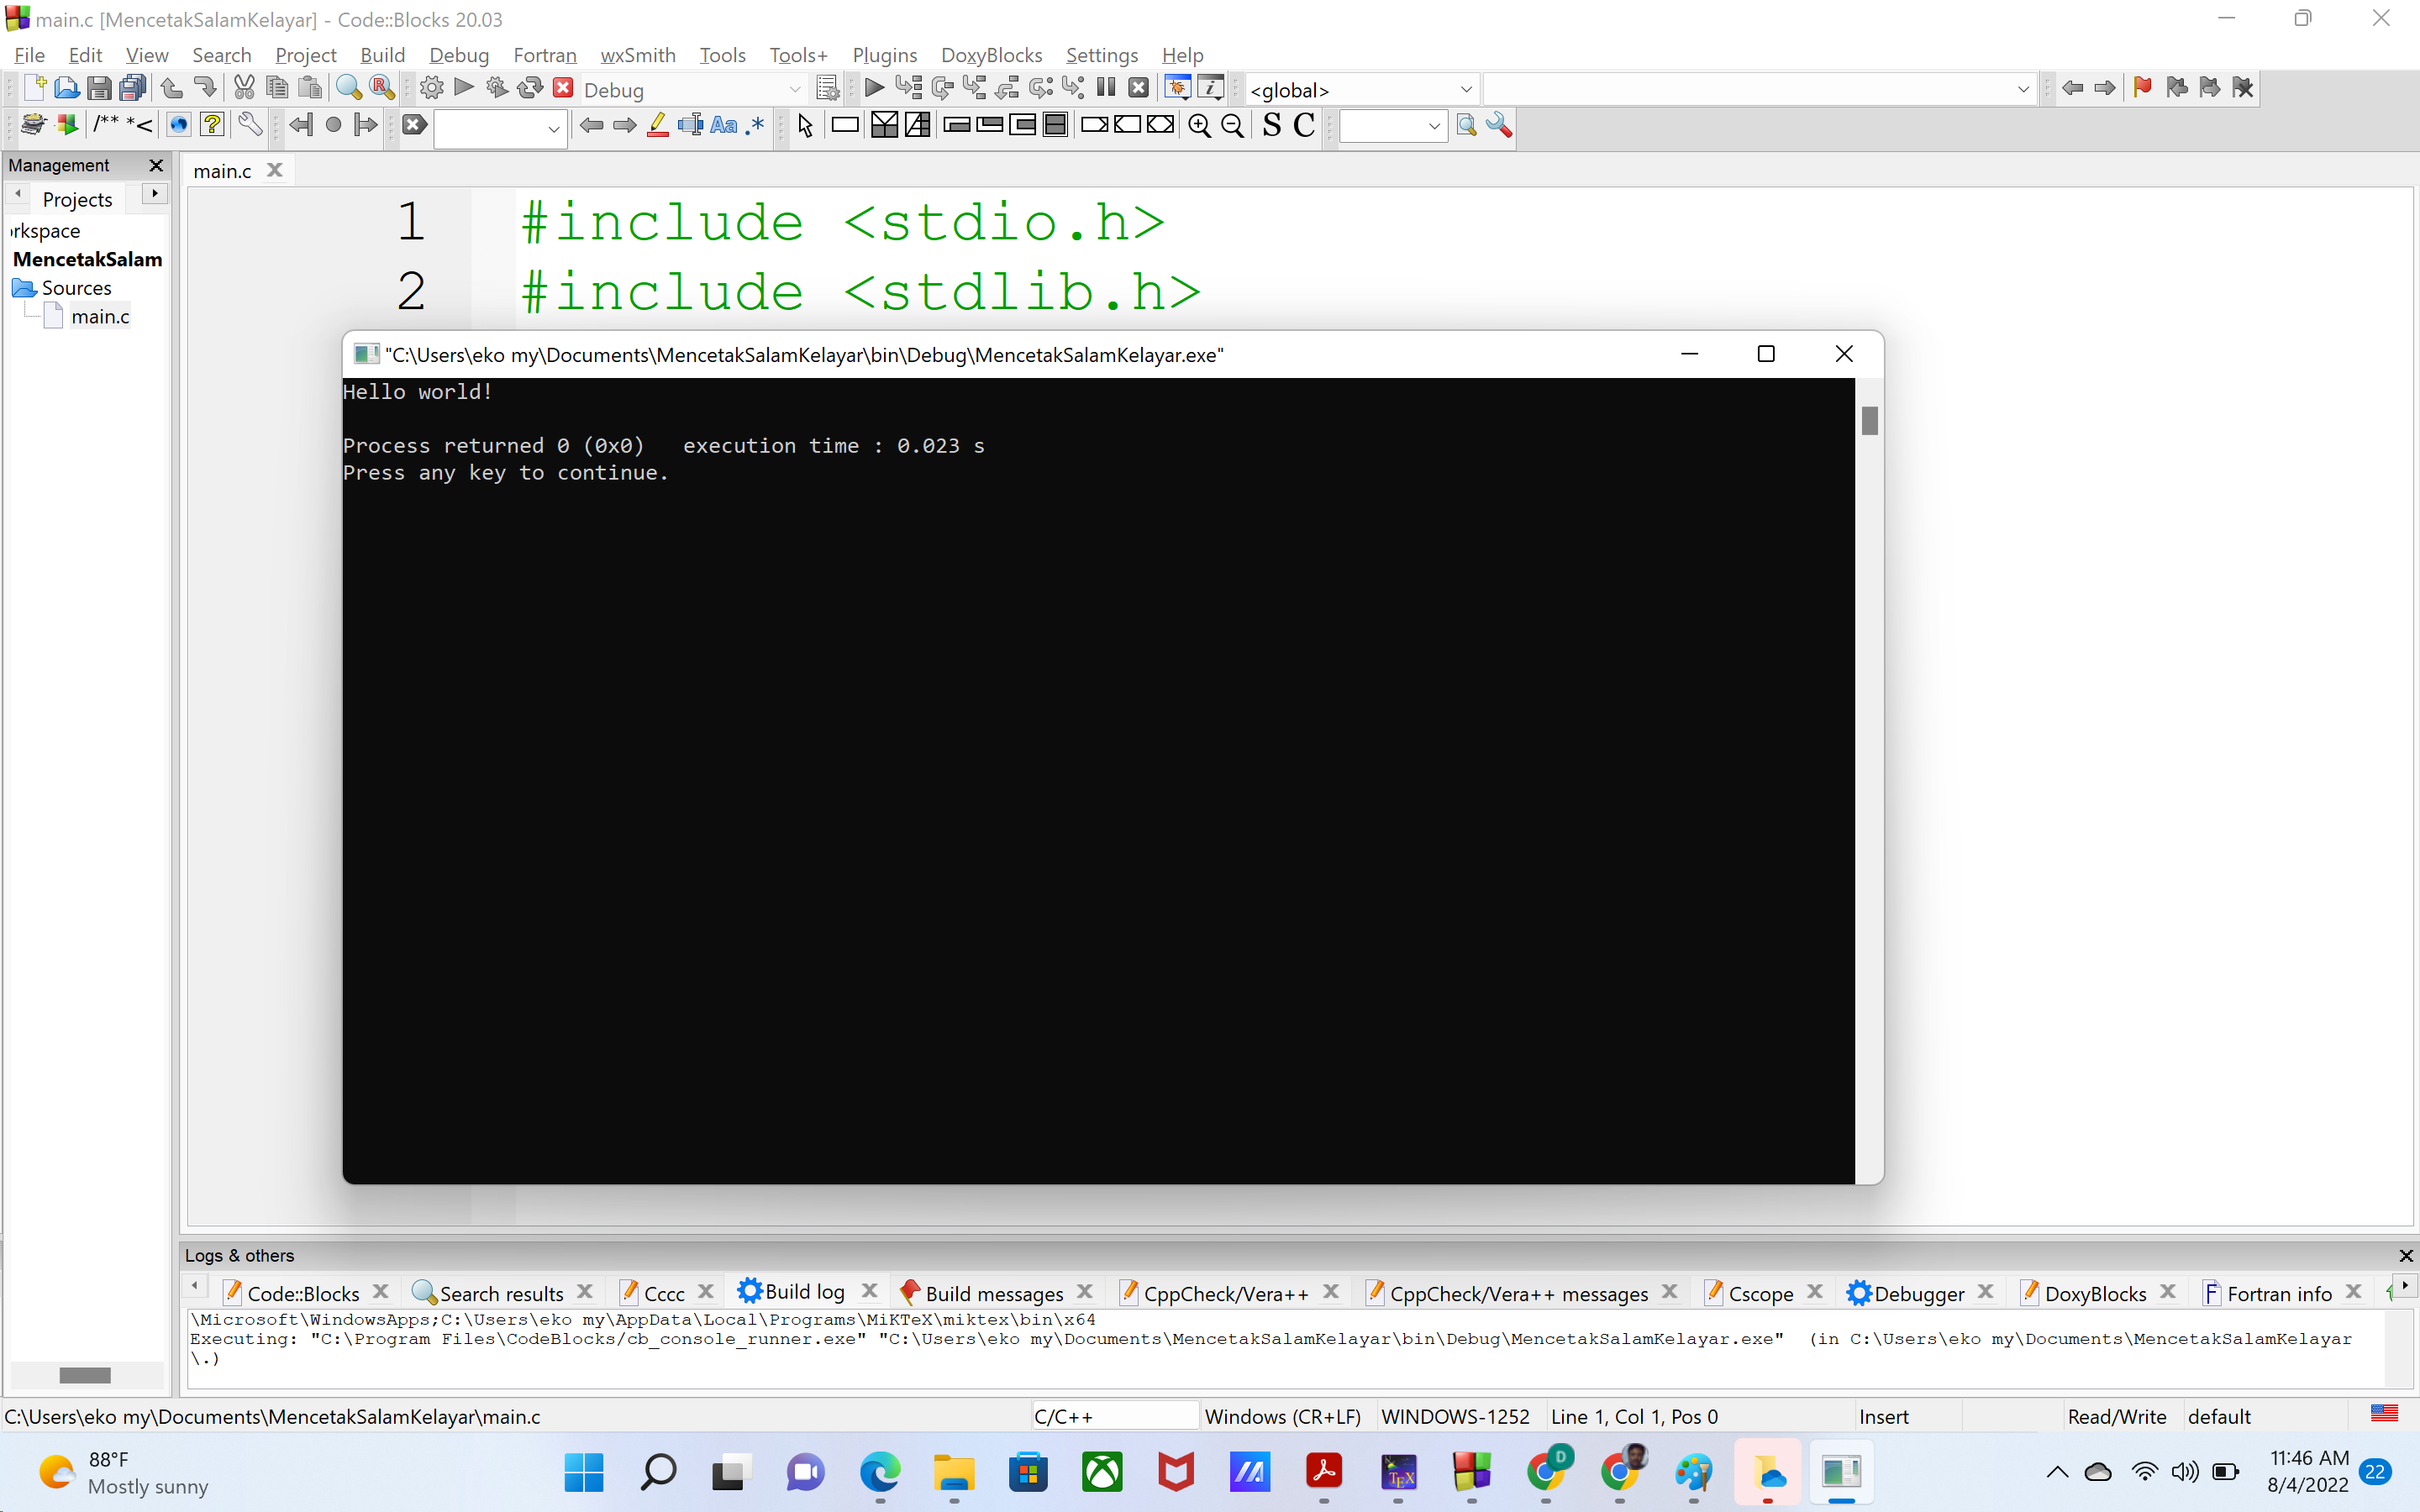
\includegraphics[width=0.7\linewidth]{P1/img/screenshot010.png}
		      \caption{}
		      \label{fig:screenshot010}
	      \end{figure}
\end{enumerate}

% \subsection{Pre-lab Assignment}
% Create a project with name HaloDunia and write the program like can be seen on figure \ref{fig:screenshot008} but change \verb|Hello World!| with \verb|Halo Dunia!|
\subsection{Pre-lab Assignment}
\begin{enumerate}
	\item Create a project with name HaloDunia and write the program like can be seen on figure \ref{fig:screenshot008} but change \verb|Hello World!| with \verb|Halo Dunia!|
\end{enumerate}

%\begin{enumerate}
%	\item  Membuat program untuk menampilkan tulisan ke layar.\\
%	Langkah-langkah
%	\begin{enumerate}
%		\item Buatlah project baru dengan nama :\verb*|MencetakTextKeLayar|
%		\item Ketiklah ulang kode pada Listing \ref{lst:mencetaksalamkelayar}
%		\begin{figure}[H]
%		\begin{lstlisting}[language=c,label=lst:mencetaksalamkelayar,caption=Mencetak Teks Kelayar,captionpos=t]
%			/*Mencetak Text ke layar*/
%			
%			#include <stdio.h>
%			
%			int main()
%			{
%				//Mencetak ke layar
%				printf("Saya belajar  Pemprograman Komputer\n");
%				return 0;
%			}
%			
%		\end{lstlisting}
%	\end{figure}
%	\end{enumerate}
%\end{enumerate}
% \section{Structure of C Programming Language}
\section{Structure of C Programming Language}

\begin{lstlisting}[language=c,caption=Simple program example for C programming language,label=lst:helloworld,captionpos=t]
#include <stdio.h>

int main()
{
	//printing to screen
	printf("Halo World");
	return 0;
}
\end{lstlisting}

% Code on Listing \ref{lst:helloworld} is a simple program to print "Halo Dunia" to screen. The following is the explanation what each line of code do in the program.
Code on Listing \ref{lst:helloworld} is a simple program to print "Halo Dunia" to screen. The following is the explanation what each line of code do in the program.
\begin{itemize}\setlength\itemsep{-0.1em}
	\item [Row 1 :] \verb|#include <stdio.h>|\\ header file library for input and output functions like \verb|printf()| (the one used on line 6)
	\item[Row 2 :] Empty line.
	\item [Row 3 :] \verb|int main()|\\ The main function. The main function is the first function to be ran when the program starts.
	\item[Row 4 :] \{ \\Beginning of the \verb|main()| function code block.
		\item[Row 5 :]\verb|//printing to screen|\\ Comments. Comments are used to explain what the program is doing. Comments are ignored by the program, but helps the reader.
		\item[Row 6 :]\verb|printf("Halo Dunia");|\\ Printing "Halo Dunia" to the screen.
	\item[Row 7 :] \verb|return 0;| \\Returning the \verb|main()| function (A function ends when it returns)
	\item [Row 8 :] \}\\Closing the \verb|main()| function code block.

	      % \item [Baris 1 :] \verb|#include <stdio.h>|\\ file library header untuk fungsi input dan output seperti \verb|printf()| (contoh digunakan di baris 6)
	      % \item[Baris 2 :] Baris kosong. 
	      % \item [Baris 3 :] \verb|int main()|\\ Fungsi main. Fungsi utama adalah fungsi pertama yang akan dijalnkan ketika program dimulai.
	      % \item[Baris 4 :] \{ \\Permulaan dari \verb|main()| fungsi code block.
	      % \item[Baris 5 :]\verb|//printing to screen|\\ Komen. Komen digunakan untuk menjelaskan program. Komen akan diabaikan oleh program, tetapi membantu pembaca.
	      % \item[Baris 6 :]\verb|printf("Halo Dunia");|\\ Print/mencetak "Halo Dunia" ke layar.
	      % \item[Baris 7 :] \verb|return 0;| \\Mengembalikan \verb|main()| fungsi (sebuah fungsi berakhir ketika dikembalikan/return)
	      % \item [Baris 8 :] \}\\Menutup \verb|main()| fungsi code block.

\end{itemize}
% \subsection{Pre-lab Assignment}
% Try to swap line 6 and line 7 in Listing \ref{lst:helloworld}. What happened?\\
% What if \verb|return 0;| replaced with \verb|return 1;|?
\subsection{Pre-lab Assignment}
\begin{enumerate}
	\item Try to swap line 6 and line 7 in Listing \ref{lst:helloworld}.Explain what happened?
	\item What if \verb|return 0;| replaced with \verb|return 1;|?
\end{enumerate}


\section{Data Types and Variable}
\subsection{Data Types}
In C programming language, there are several data types to represent integer, real number, characters, string, and etc.
% In C programming language, there are several data types to represent integer, real number, characters, string, and etc.
\begin{center}

	\captionof{table}{Some data types in C programming language \label{tab:tipedata}}
	\begin{tabular}{|l|l|l|}
		\hline
		Data Types                     & Size     & Range Value                     \\ \hline
		Int (or signed int)            & 2 bytes  & -32,768 to 32,767               \\ \hline
		unsigned int                   & 2 bytes  & 0 to 65,535                     \\ \hline
		Short int(or signed short int) & 2 bytes  & -32,768 to 32,767               \\ \hline
		Long(or singed short int)      & 4 bytes  & -2,147,483,648 to 2,147,483,647 \\ \hline
		unsigned long                  & 4 bytes  & 0 to 4,294,967,295              \\ \hline
		float                          & 4 bytes  & 1.2E-38 to 3.4E+38              \\ \hline
		double                         & 8 bytes  & 2.3E-308 to 1.7E+308            \\ \hline
		Long double                    & 10 bytes & 3.4E-4932 to 1.1E+4932          \\ \hline
		char(or signed char)           & 1 byte   & -128 to 127                     \\ \hline
		unsigned char                  & 1 byte   & 0 to 255                        \\ \hline

		%     \captionof{table}{Beberapa tipe data di C \label{tab:tipedata}}
		% 	% \begin{tabular}{|l|l|l|}
		% 	% 	\hline
		% 	% 	Data Types & Size         & Description                                         \\ \hline
		% 	% 	int       & 2 or 4 bytes & saves integers                        \\ \hline
		% 	% 	float     & 4 bytes      & saves real numbers to 8 digit behind decimal point. \\ \hline
		% 	% 	double    & 8 bytes      & saves real numbers to 15 digits behind decimal point. \\ \hline
		% 	% 	char      & 1 byte       & saves a character                     \\ \hline
		% 	% \end{tabular}
		% 	\begin{tabular}{|l|l|l|}
		% 		\hline
		% 		Tipe Data & Ukuran       & Deskripsi                                         \\ \hline
		% 		int       & 2 atau 4 bytes & menyimpan integers.                        \\ \hline
		% 		float     & 4 bytes      & menyimpan bilangan real (8 digit dibelakang desimal). \\ \hline
		% 		double    & 8 bytes      & menimpan bilangan real (15 digit dibelakang desimal). \\ \hline
		% 		char      & 1 byte       & menyimpan sebuah karakter.                     \\ \hline
	\end{tabular}
\end{center}
% Untuk menampilkan data pada layar, setiap tipe data memiliki format specifier yang dapat digunakan pada formatted string. Berikut adalah format specifier untuk beberapa tipe data.
To show the data on screen, every data type has a format specifier that can be used on formatted string. The following is the format specifier for several data types.
\begin{center}
	\captionof{table}{Format Specifier \label{tab:formatspecifier}}
	\begin{tabular}{|l|l|}
		\hline
		Format Specifier & Data Types \\ \hline
		\%d or \%i       & int        \\ \hline
		\%f              & float      \\ \hline
		\%lf             & double     \\ \hline
		\%c              & char       \\ \hline
		\%s              & string     \\ \hline
	\end{tabular}
\end{center}
% Masih ada lebih banyak tipe data dari pada yang dituliskan pada Tabel \ref{tab:tipedata}. Tipe-tipe data ini dan spesifikasinya bisa ditemukan dengan mudah di internet.
There are still more data types that what was written on Table \ref{tab:tipedata}. These data types and its specification can be found easily on the internet.

\subsubsection{Modifier}
In general, a modifier is a word, phrase, or clause that modifies or describes a noun or verb in a sentence. Meanwhile, in programming languages, a modifier is a keyword used to alter the behavior or characteristics of an element in a program, such as variables, functions, or classes. We use modifiers to change the range of basic data types to fit programming needs. There are four modifiers, namely:
\begin{enumerate}
	\item signed \\
	      \verb|int value = -10;| (Using a negative sign for variables of type int, which are signed integers by default.)
	\item unsigned \\
	      \verb|unsigned int count = 100;|  (Using a negative sign for variables of type int, which are signed integers by default.)
	\item long \\
	      \verb|long population = 7500000000;| (Using the long data type to store values larger than the int data type.)
	\item short \\
	      \verb|short temperature = 20;| (Using the short data type to save memory when we know that the values to be stored will be relatively small.)
\end{enumerate}


\subsection{Variable}
Variables are places to store data. Declaring a variable can be done in the following ways
\begin{lstlisting}[language=c,caption=C variable declaration,label=lst:deklarasivariabel,captionpos=t]
DataType VariableName;
\end{lstlisting}
\subsubsection{Aithmetic and Assignment Operator }
Assignment operator can be use in variabel that is not a \verb*|const| or a varable that has -1 value. However, arithmetic operators can accept both variables with 'const' or without ('left-hand' and 'right-hand' values)
The table below shows some arithmetic operators in C
\begin{center}
	\captionof{table}{Arithmetic operator in C programming language\label{tab:operatoraritmatika}}
	\begin{tabular}{|c|l|c|}
		\hline

		\multicolumn{1}{|l|}{Operator} & Name           & \multicolumn{1}{l|}{Example} \\ \hline

		% 		\multicolumn{1}{|l|}{\textbf{Operator}} & \textbf{Nama} & \multicolumn{1}{l|}{\textbf{Contoh}} \\ \hline

		+                              & Addition       & \verb|x + y |                \\ \hline
		-                              & Subtraction    & \verb|x = y|                 \\ \hline
		*                              & Multiplication & \verb|x * y|                 \\ \hline
		/                              & Distribution   & \verb|x/y|                   \\ \hline
		\%                             & Modulo         & \verb|x % y|                 \\ \hline
	\end{tabular}
\end{center}

% Tabel di bawah menunjukkan beberapa operator penugasan.
\begin{center}
	\captionof{table}{Assignment operator \label{tab:operatorpenugasan}}
	\begin{tabular}{|c|c|c|}
		\hline
		\multicolumn{1}{|l|}{Operator} & \multicolumn{1}{l|}{Example}      & \multicolumn{1}{l|}{Similiar meaning} \\ \hline
		=                              & x = 5                             & x = 5                                 \\ \hline
		+=                             & x += 3                            & x = x + 3                             \\ \hline
		-=                             & x -= 3                            & x = x - 3                             \\ \hline
		*=                             & x *= 3                            & x = x * 3                             \\ \hline
		/=                             & x /= 3                            & x = x / 3                             \\ \hline
		\%=                            & x \%= 3                           & x = x \% 3                            \\ \hline
		\&=                            & x \&= 3                           & x = x \& 3                            \\ \hline
		|=                             & x |= 3                            & x = x | 3                             \\ \hline
		\textasciicircum{}=            & x \textasciicircum{}= 3           & x = x \textasciicircum 3              \\ \hline
		\textgreater{}\textgreater{}=  & x \textgreater{}\textgreater{}= 3 & x = x \textgreater{}\textgreater 3    \\ \hline
		\textless{}\textless{}=        & x \textless{}\textless{}= 3       & x = x \textless{}\textless 3          \\ \hline
	\end{tabular}
\end{center}
There are also 'abbreviations' for some assignment operators such as \verb*|x+=1| and \verb*|x-1|, which \verb*|++| and \verb*|--|. There are also 'abbreviations' for some assignment operators such as.
\begin{verbatim}
    x++;
    x--;
    ++x;
    --x;
\end{verbatim}

\subsubsection{Operator Bitwise}
Bitwise operators are special operators used to handle logical operations on binary numbers in bit form. Binary numbers themselves are a type of number consisting of only two digits, which are 0 and 1. If the original value used is not in binary, it will be automatically converted by the C compiler into a binary number. For example, 7 in decimal equals 0111 in binary
\\
\begin{center}
	\captionof{table}{Bitwise operator\label{tab:operatorbitwise}}
	\begin{tabular}{|c|c|c|c|c|c|}
		\hline
		\multicolumn{1}{|l|}{Operator} & \multicolumn{1}{|l|}{Name} & \multicolumn{1}{|l|}{Example}   & \multicolumn{1}{|l|}{Binary}      & \multicolumn{1}{|l|}{Result (binary)} & \multicolumn{1}{|l|}{Result (decimal)} \\ \hline
		\&                             & AND                        & 10 \& 12                        & 1010 \& 1100                      & 1000                                  & 8                                      \\ \hline
		|                              & OR                         & 10 | 12                         & 1010 | 1100                       & 1110                                  & 14                                     \\ \hline
		\textasciicircum{}             & XOR                        & 10 \textasciicircum 12          & 1010 \textasciicircum 1100        & 0110                                  & 6                                      \\ \hline
		$\sim$                         & NOT                        & $\sim$10                        & $\sim$1010                        & 0101                                  & -11 (two complement)                   \\ \hline
		\textless{}\textless{}         & Left shift                 & 10 \textless{}\textless 1       & 1010 \textless{}\textless 1       & 10100                                 & 20                                     \\ \hline
		\textgreater{}\textgreater{}   & Right shift                & 10 \textgreater{}\textgreater 1 & 1010 \textgreater{}\textgreater 1 & 101                                   & 5                                      \\ \hline
	\end{tabular}
\end{center}

\begin{center}
	\colorbox{pink}{\parbox{0.8\linewidth}{\textbf{Notes:} There are several operators in the C language. Please study them by seeking references independently}}
\end{center}
\subsection{Pre-lab Assignment}
\begin{lstlisting}[language=c,caption=Using assignment operator in a const variable,label=lst:constassignment,captionpos=t]
#include <stdio.h>
int main()
{

	//variable declaration
    const int x=0;
    x=1;
	return 0;
}
\end{lstlisting}
Try to compile the program in Listing\ref{lst:constassignment}, what happened?
% Coba jalankan program di Listing \ref{lst:constassignment}, apa yang terjadi?


\section{Input and Output}

\subsection{printf()}
\verb*|printf| is a function in C that is used to print formatted string.  You can use format specifier \verb*|%| within the formatted string to outputs your variables.
% is a function in C that is used to print formatted string.
% You can use format specifier within the formatted string to outputs your variables.

\begin{verbatim}
	printf(const char *format,v1,v2,..,vn)
\end{verbatim}

% Format specifier untuk beberapa tipe data dapat dilihat pada Tabel \ref{tab:formatspecifier}
The format specifier for each data types can be seen on Table \ref{tab:formatspecifier}


\begin{description}
	\item[Contoh \thesubsection.1]  Printing text to the screen.
		\begin{lstlisting}[language=c,caption = Print text "C Programming" Ke layar,captionpos=t]
		#include <stdio.h>    
		int main()
		{ 
			// Printing text inside the " symbol
			printf("C Programming");
			return 0;
		}
	\end{lstlisting}
		\begin{itemize}
			% \item Seluruh program C harus berisi fungsi main() tempat program memulai menjalankan kode. 
			\item All C program must have main() function where the program needs to run the code.
			      % \item Fungsi \verb*|printf()| adalah library untuk mengirim output yang telah diformat ke layar.  Fungsi \verb*|printf()|  mencetak string dalam tanda dua tanda petik. 
			\item \verb*|printf()| function is a function from stdio.h library. This function outputs the string inside the symbol " to the screen.
			\item \verb*|return 0;| statement in the \verb*|main()| function tells the program to exit.
			\item \verb*|return 0;| pernyataan di \verb*|main()| fungsi memberitahu program untuk keluar.
		\end{itemize}
	\item [Contoh \thesubsection.2] Printing integer.
	      \begin{lstlisting}[language=c,captionpos=t]
		#include <stdio.h>
		int main()
		{
			int testInteger = 5;
			printf("Number = %d", testInteger); // <- %d format string
			return 0;
		}
	\end{lstlisting}


	      % Pada contoh ini digunakan format specifier \verb*|%d| untuk mencetak tipe data \verb*|int|. \verb*|%d| pada tex akan digantikan oleh isi dari \verb*|testInteger|. 
	      The code above uses the format specifier \verb*|%d| to prints \verb*|int| data type. The \verb*|%d| part of the string will be replaced with the value of \verb*|testInteger|.

	\item[Contoh \thesubsection.3] Real number output (float atau double)
		\begin{itemize}\label{eq:LuasSegitiga}
			\item \verb|Base|  : using \verb|float| data type.
			\item \verb|Height|: using \verb|float| data type.
			\item \verb|Area|  : using \verb|float| data type.
			      \begin{equation}
				      Area = \frac{1}{2} \times Base \times Height
			      \end{equation}
		\end{itemize}
		\begin{lstlisting}[language=c,captionpos=t]
		#include <stdio.h>
		
		int main()
		{
			// variable declaration
			float Base;
			float Height;
			float Area;
			// value initialization
			Base = 10;
			Height = 5;
			// calculating area
			Area = 0.5*Base*Height;
			// printing the text to screen
			printf("Area = %f",Area);
			return 0;
		}
		
	\end{lstlisting}

		explanation
		\begin{description}
			\item[Row 6-8]  \verb|Base|, \verb|Height| and \verb|Area| are \verb|float|data type which use to store triangle area data.
			\item[Row 10 dan 11] Value initialization to \verb|Base|=10 and \verb|Height|=5
			\item[Row 13] Calculating triangle area according to  the equation \ref{eq:LuasSegitiga}
			\item[Row 15] Printing \verb|Area| to the screen using \verb|printf| command.
		\end{description}
\end{description}

.\subsection{scanf}
Function \verb*|scanf(const char *format, ...)| reads input according to the format string.
% \verb*|scanf(const char *format, ...)| reads input according to the format string.

\begin{enumerate}
	\item Syntax
	      \begin{verbatim} scanf(const char *format, ...)
	\end{verbatim}
	\item Parameter \\
	      Format string in C consist of one or more whitespace, non-whitespace, and format specifiers.
	      % Format string pada C yang terdiri dari satu atau lebih yang terdiri dari \\
	      % Karakter Whitespace,Karakter Non-whitespace  dan  Format specifiers. 
	\item Return Value \\
	      % Ketika berhasil maka fungsi mengembalikan jumlah item dari argumen yang berhasil di baca.
	      The function will return the number of arguments it has sucessfully read.

\end{enumerate}

\begin{description}
	\item  [Example \thesubsection.4] Calculating triange \verb*|Base|   dan tinggi \verb*|Height| yang diinputkan dari keyboard.
	      \begin{lstlisting}[language=c]
#include <stdio.h>

int main()
{
	float Base, Height, Area;
	
	printf("Calculate triangle area\n");
	printf("\Insert Base= ");
	scanf("%f",&Base);
	printf("\nMasukkan Height=");
	scanf("%f",&Height);
	Area = 0.5*Base *Height;
	printf("Triangle Area = %.2f", Area);
	return 0;
}
	\end{lstlisting}
	      \begin{figure}[H]
		      \centering
		      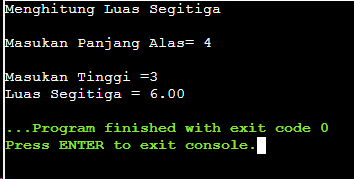
\includegraphics[width=0.5\linewidth]{P1/img/screenshot0005.png}
		      \caption{}
		      \label{fig:screenshot0005}
	      \end{figure}

	      \begin{description}
		      \item [Row 9]\verb|scanf("%f",&Area);| requesting input for triangle base
		      \item [Row 11]\verb|scanf("%f",&Height);| requesting input for triangle height
		      \item [Row 13]\verb|printf("Triangle Area = %.2f", Area);|,  \verb|.2| si \verb|%.2f| indicating that only 2 digits after the decimal point need to be printed
	      \end{description}

	\item[Example \thesubsection.5] Program to input name and email.\\
		% Pada contoh ini dipelajari bagaimana cara menginputkan string atau text dari keyboard dan mencetak kelayar. Input dari contoh program ini ada dua yang terdiri dari \verb|snama| dan \verb|sAlamatEmail|. Oleh karena text berisi banyak karakter maka masing-masing variabel dideklarasikan sebagai kumpulan karakter dengan jumlah karakter untuk sNama=20 dan sAlamatEmail=30. 
		This example shows how to input string or text from keyboard and outputs it on the screen. Input from this program consist of \verb|sName| and \verb|sEmail|. Because the text contains many characters, each variable is declared as an array of characters with the number of characters for sName=20 and sEmailAddress=30.
		\begin{figure}[H]
			\begin{lstlisting}[language=c]
		#include <stdio.h>
		
		int main () 
		{
			char sName[20], sEmail[30];
			
			printf("Enter Name: ");
			scanf("%19s", sName);
			
			printf("Enter Email: ");
			scanf("%29s", sEmail);
			
			printf("Name : %s\n", sName);
			printf("Email:%s", sEmail);
			return(0);
		}
	\end{lstlisting}
		\end{figure}
\end{description}


\subsection{Escape Sequence}
% Escape Sequence adalah urutan karakter yang digunakan untuk memformat output dan tidak ditampilkan ketika dicetak ke layar. Setiap karakter mempunyai fungsi tertentu. 
Some characters can't be written on the format string because they are used to format the outputs. So, to outputs those special characters we use escape sequences.

\begin{table}[H]
	\centering
	\captionof{table}{Escape Sequence \label{tab:escapesequence}}
	\begin{tabular}{|l|l|l|}
		\hline
		Escape sequence                  & Output          \\ \hline
		\textbackslash{}a                & Bell, alarm     \\ \hline
		\textbackslash{}b                & Backspace       \\ \hline
		\textbackslash{}f                & Change Page     \\ \hline
		\textbackslash{}n                & Change Row      \\ \hline
		\textbackslash{}r                & Carriage return \\ \hline
		\textbackslash{}t                & Tab Horizontal  \\ \hline
		\textbackslash{}v                & Tab Vertikal    \\ \hline
		\textbackslash{}'                & Single Quotes   \\ \hline
		\textbackslash{}"                & Double Quotes   \\ \hline
		\textbackslash{}?                & Question Mark   \\ \hline
		\textbackslash{}\textbackslash{} & Backslash       \\ \hline
	\end{tabular}
\end{table}

\begin{description}
	\item[Contoh \thesubsection.6] Change row with escape sequence \verb*|\n|.
		\begin{lstlisting}
#include <stdio.h>

int main() 
{
	printf("Halo \nI'm learning C programming language.\nand it's so fun!");
	return 0;
}
	\end{lstlisting}
		\begin{figure}[H]
			\centering
			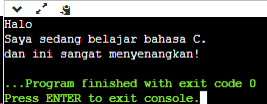
\includegraphics[width=0.5\linewidth]{P1/img/screenshot0006.png}
			\caption{}
			\label{fig:screenshot0006}
		\end{figure}

	\item[Contoh \thesubsection.7] Using escape sequence\verb*|\t| to change tab.
		\begin{lstlisting}[language=c]
#include <stdio.h>
int main(void)
{
	printf("Name \t\t: Rahmad Rahardi\n");
	printf("Address \t\t: Bendungan Hilir Jakarta\n");
	printf("Place of Birth \t: Jakarta\n");
	printf("Date of Birth \t: 30 February 2000\n");
	
	return (0);
}
\end{lstlisting}
		\begin{figure}[H]
			\centering
			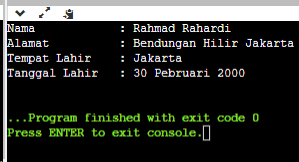
\includegraphics[width=0.5\linewidth]{P1/img/screenshot0007.png}
			\caption{}
			\label{fig:screenshot0007}
		\end{figure}
\end{description}

\subsection{Pre-lab Assignment}
\begin{enumerate}
	\item Try to build a program to read input for the name and NRP and display it to the screen.
	\item Try to build a program that asks user to enter a Celcius temperature and then convert it to Farenheit.  .
\end{enumerate}

\begin{center}
	\colorbox{cyan!30}{\parbox{0.8\linewidth}{\textbf{Optional:} Learn Git and Github. You can start learning from the following resources: \\ \href{https://github.com}{GitHub - https://github.com} \\ \href{https://git-scm.com/doc}{Git -https://git-scm.com/doc}}}
\end{center}
% \section{Goals}
\begin{itemize}[label=$\bullet$, itemsep=-1pt, leftmargin=*]
	\item Students are familiar with and able to use logical and comparison expressions in the C programming language.
	\item Students are familiar with and able to use logical and comparison expressions in the C programming language.
	\item Students can recognize and use while loops in the C language.
	      % \item Students are able to use while-loop on C
	\item Students can recognize and use do-while loops in the C language.
	      % \item Students are able to use do-while loop on C
	\item Students can recognize and use for loops in the C language.
	      % \item Students are able to use for loop on C
	\item Students can recognize and use for loops in the C language.
	      % \item Students are able to use one dimensional or multidimensional array
	\item Students can recognize and use for loops in the C language.
	      % \item Students are able to use loops to process data on arrays
	\item Students can recognize and use strings.
\end{itemize}
\section{Logical and Comparasion Expressions}
\subsection{Comparasion Expressions}
% Berikut adalah operator-operator yang digunakan pada suatu ekspresi perbandingan
The following are the operators used in comparison expressions.
\begin{center}
	\captionof{table}{Comparasion Operator\label{tab:operatorcomp}}
	\begin{tabular}{|c|l|c|}
		\hline
		\textbf{Operator} & \textbf{Name}         & \multicolumn{1}{l|}{\textbf{Expression Example}} \\ \hline
		!=                & Not Equal To          & x != y                                           \\ \hline
		\textgreater{}    & Greater Than          & x \textgreater y                                 \\ \hline
		==                & Equal To              & x == y                                           \\ \hline
		\textless{}       & Less Than             & x \textless y                                    \\ \hline
		\textgreater{}=   & Greater Than Equal To & x \textgreater{}= y                              \\ \hline
		\textless{}=      & Less Than Equal To    & x \textless{}= y                                 \\ \hline
	\end{tabular}
\end{center}

% Suatu ekspresi perbandingan akan mengembalikan nilai berupa \verb|true| atau \verb|false| yang ditandakan dengan nilai 0 atau 1.
A Comparison Expression will return boolean value \verb|true| or \verb|false| which is also represented with the value of 0 or 1.
As example:
\begin{verbatim}
    printf("%d",0>1); // Print 0 to the screen
    printf("%d",0<1); // Print 1 to the screen
\end{verbatim}

\subsection{Logical Expression}
% Berikut adalah operator-operator logika yang digunakan pada suatu ekspresi logika
The following are the logical operators used on a Logical Expression
\begin{center}
	\captionof{table}{Logical Expression \label{tab:operatorlogic}}
	\begin{tabular}{|c|l|c|}
		\hline
		\textbf{Operator} & \multicolumn{1}{c|}{\textbf{Name}} & \textbf{Expression Example} \\ \hline
		$\&\&$            & AND                                & $x<5\; \&\& \;x<10$         \\ \hline
		$||$              & OR                                 & $x < 5\; ||\; x < 4  $      \\ \hline
		$!$               & NOT                                & $!(x <5 \&\& x < 10) $      \\ \hline
	\end{tabular}
\end{center}
% Sama seperti ekspresi perbandingan, ekspresi logika akan mengembalikan nilai berupa true atau false
Like comparison expression, logical expression will return boolean values.

\section{Branch}
\subsection{If Statement}
\verb*|if| statement is used to decide which block of code to be executed if the condition is true.
% \verb*|if| digunakan untuk menentukan blok kode C yang dijalankan apabila ekspresi kondisi bernilai benar (TRUE),
\begin{verbatim}
// Block code before if
if (Condition) 
{
 // Block of code that will be executed if the condition is true
}
// Block code after if
\end{verbatim}
% Sebagai contoh, perhatikan program berikut
As example, look at the following code
\begin{lstlisting}[language=c,caption =If Statement Example,label=lst:ifexample01]
	include <stdio.h>
	
	int main()
	{
		//Variable Declaration
		int myMoney,breadPrice;
		myMoney = 5000;
		breadPrice = 10000;
		
		if (myMoney>=breadPrice)
		{
		    printf("I can buy that bread\n");
		}
		printf("hehe");
		return 0;
	}
\end{lstlisting}
Output of the program
\begin{verbatim}
    hehe
\end{verbatim}
If line 7 changed to \verb|myMoney=10000|, the outputs of the program would be
% Jika baris ke 7 diganti dengan \verb|myMoney=10000| maka output dari program ini akan menjadi
\begin{verbatim}
    I can buy that bread
    hehe
\end{verbatim}

\subsection{If-else Statement}
% Pernyataan else digunakan untuk menentukan blok kode yang di jalankan apabila kondisi salah. 
\verb|Else| statement is used to decide the block of code to be executed if the condition is false.
\begin{verbatim}
// Block code before if
if (Condition) 
{
	// Block of code that will be executed if the condition is true
} else
{
	// Block of code that will be executed if the condition is false
}
// Bloc code after if-else
\end{verbatim}
% Berikut contoh penggunaan if-else
The following is an example of using if-else statement:
\begin{lstlisting}[language=c,caption = If-else example,label=lst:ifelseexample01]
	include <stdio.h>
	
	int main()
	{
		//Varible declaration
		int myMoney,breadPrice;
		myMoney = 5000;
		breadPrice = 10000;
		
		if (myMoney>=breadPrice)
		{
		    printf("I can buy that bread\n");
		}
		else
		{
	        printf("I can't buy that bread\n");	
		}
		printf("hehe");
		return 0;
	}
\end{lstlisting}
Below is the output of that program
\begin{verbatim}
    I can buy that bread
    hehe
\end{verbatim}
%  \verb|myMoney=10000| maka output dari program ini akan menjadi
If line 7 changed to \verb|myMoney=10000|, the outputs of the program would be
\begin{verbatim}
    I can't buy that bread
    hehe
\end{verbatim}

\subsection{Pernyataan if-else if}
% Statement \verb|else if| digunakan untuk menjalankan blok kode apabila kondisi statement \verb|if| atau \verb|else if| sebelumnya bernilai salah.
The \verb|else if| statement is used to run a block of code when the condition in \verb|if| or the previous \verb|else if| is false.
\begin{verbatim}
	// Code block before the if statement
if (Condition1)
{
    /* Code block to be executed if Condition 1
    is true */
}
else if (Condition2)
{
    /* Code block to be executed if Condition 1 is false
    and Condition 2 is true */
}
else if (Condition3)
{
    /* Code block to be executed when
    Condition 1 and Condition 2 are false, and
    Condition 3 is true */
}
...
else if (ConditionN)
{
    /* Code block to be executed when
    Condition 1 to Condition N-1 are false, and
    Condition N is true */
}
else
{
    /* Code block to be executed when
    Condition 1 to Condition N are false */
}
// Code block after the if statement
\end{verbatim}
Below are an example of if-else statement
\begin{lstlisting}[language=c,caption = If-else example if,label=lst:ifelseifexample01]
	include <stdio.h>
	
	int main()
	{
		//Varible declaration
		int myMoney,breadPrice;
		myMoney = 5000;
		breadPrice = 10000;
		
		if (myMoney>breadPrice)
		{
		    printf("I can buy that bread\n");
		}
		else if(myMoney==breadPrice)
		{
		    printf("I can buy bread, but my money will run out immediately");
		}
		else
		{
	        printf("I can't buy that bread\n");	
		}
		printf("hehe");
		return 0;
	}
\end{lstlisting}
Output of this program are below
\begin{verbatim}
    I can't buy that bread
    hehe
\end{verbatim}
% Jika baris ke 7 diganti dengan \verb|myMoney=10000| maka output dari program ini akan menjadi
If line 7 changed to \verb|myMoney=10000|, the output of the program would be
\begin{verbatim}
    I can buy bread, but my money will run out immediately
    hehe
\end{verbatim}
% Jika baris ke 7 diganti dengan \verb|myMoney=12000| maka output dari program ini akan menjadi
If line 7 changed to \verb|myMoney=12000|, the output of the program would be
\begin{verbatim}
    I can buy that bread
    hehe
\end{verbatim}

\subsection{Nested if}
% Nested if merupakan konsep di mana di dalam suatu blok if terdapat statement if.
Nested if is when there is a conditional statements within a block of code inside the conditional statement
\begin{verbatim}
	// Code block before the if statement
	if (Condition1) 
	{
		if (Condition2)
		{
			// Do something
		}
		else
		{
			// Do other thing
		}
	} 
	else
	{
		// Do other thing
	}
\end{verbatim}

% Berikut contoh penggunaan nested if
Below is an example of using nested if

\begin{lstlisting}[language=c,caption = Nested if example,label=lst:nestedifexample01]
	include <stdio.h>
	
	int main()
	{
		// Declare the variables
		int myMoney,breadPrice,friendsMoney;
		myMoney = 5000;
		breadPrice = 10000;
		friendsMoney = 42069;
		
		
		if (myMoney>breadPrice)
		{
		    printf("I can buy bread\n");
		}
		else if(myMoney==breadPrice)
		{
		    printf("I can buy bread but I will ran out of money\n");
		}
		else
		{
		    if(friendsMoney+myMoney >= breadPrice)
		    {
		        printf("I can buy bread if I borrow my friend money\n"); 
		    }
		    else
		    {
	            printf("I can't buy bread\n");	
		    }
		}
		printf("hehe");
		return 0;
	}
\end{lstlisting}


\subsection{Pre-lab Assignment}
\begin{enumerate}
	\item what is the purpose of branching in programming?
	\item Apart from using if statements, branching can also be done using switch-case statements. Explain what you know about switch-case statement!
	% \item Buatlah program yang menerima input 3 buah bilangan bulat A, B, dan C. Outputkanlah 3 bilangan bulat itu ke layar dengan urutan paling kecil ke paling besar. Lakukanlah ini dengan menggunakan statement if, if else, if else if, atau nested if.
	\item Try to make a program that receives 3 integer input A, B, and C. Then outputs those 3 integers to the screen sorted from largest to smallest. Do this only using conditional statements.
\end{enumerate}

\section{Loop}
\subsection{Loop while}
% Perulangan while akan menjalankan blok kode yang berada di dalamnya selama kondisi perulangan masih bernilai benar.
While loop will run the code block within it repeatedly as long as the loop condition is true


\begin{figure}[H]
	\centering
	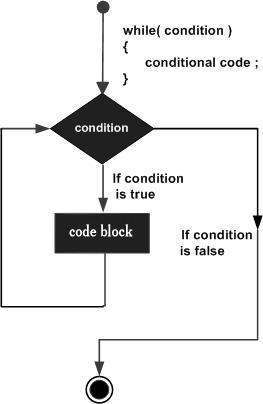
\includegraphics[width=0.4\linewidth]{P2/img/whileloop.png}
	\caption{Flow chart loop while}
	\label{fig:whileloop}
\end{figure}

% Syntaxnya pada bahasa C adalah sebagai berikut:
Its syntax in C programming language is as follows
\begin{verbatim}
    while(Condition)
    {
        // Block of code that will be repeated
    }
\end{verbatim}

% Sebagai contoh, perhatikan kode berikut
As an example, look at the following code
\begin{lstlisting}[language=c,caption = While implementation example,label=lst:whileexample01]
int main()
{
	int myMoney,breadPrice;
	myMoney = 10000;
	breadPrice = 2000;
	while(myMoney >= breadPrice)
	{
	    printf("Buy 1 bread, my money left %d", myMoney - breadPrice);
	    myMoney -= breadPrice;
	}
	printf("I don't have enough money");
	return 0;
}
\end{lstlisting}
Output in program \ref{lst:whileexample01} are below
\begin{verbatim}
    Buy 1 bread, my money left 8000
    Buy 1 bread, my money left 6000
    Buy 1 bread, my money left 4000
    Buy 1 bread, my money left 2000
    Buy 1 bread, my money left 0
    I don't have enough money
\end{verbatim}

% Pada contoh ini, operasi pada baris 9 membuat variabel \verb|myMoney| berkurang 2000 pada setiap pengulangan hingga akhirnya nilai \verb|myMoney| tidak lebih dari atau sama dengan \verb|breadPrice| lagi.
You can see the line 9 of the code causes the variable \verb|myMoney| to have its value substracted by 2000 for every loop until \verb|myMoney| is no longer greater than equal to \verb|breadPrice|.
The loop condition will be invalid and finaly exits the loop. Then it prints "Uang saya tidak cukup lagi", the command after the while loop statement.
% Kondisi perulangan akan menjadi tidak valid dan akhirnya keluar dari perulangan. Kemudian ia mencetak "Uang saya tidak cukup lagi", perintah setelah pernyataan while loop.
\subsection{Do-while loop}
% do-while loop sebenarnya sama seperti while loop hanya saja do-while akan menjalankan perintah pada blok kode didalamnya terlebih dahulu sebelum melakukan pengecekan kondisi.
do-while loop is very similar to while loop. The only difference is that do-while loop will execute the code block inside it once, and then checks the condition.
\begin{figure}[H]
	\centering
	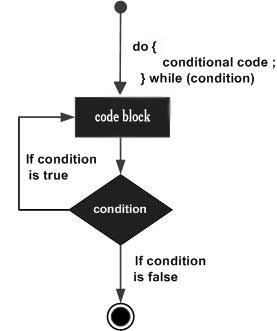
\includegraphics[width=0.4\linewidth]{P2/img/dowhileloop.png}
	\caption{Do-while statement}
	\label{fig:dowhileloop}
\end{figure}
% Syntaxnya pada bahasa C adalah sebagai berikut:
Its syntax in C is as follows:
\begin{verbatim}
    do{
        // the block of code that will be repeated
    }while(Condition)
\end{verbatim}
% Sebagai contoh, perhatikan kode berikut
Look at the following example.
\begin{lstlisting}[language=c,caption = Do-while implementation example,label=lst:dowhileexample01]
int main()
{
	int myMoney,breadPrice;
	myMoney = 10000;
	breadPrice = 12000;
	do{
	    printf("Buy 1 bread, my money left %d", myMoney - breadPrice);
	    myMoney -= breadPrice;
	}while(myMoney >= breadPrice)
	printf("Uang saya tidak cukup lagi");
	return 0;
}
\end{lstlisting}
The output of the code above in Listing \ref{lst:dowhileexample01} are
% The output of the code above are
\begin{verbatim}
    Buy 1 bread, my money -2000
    I don't have enough money
\end{verbatim}
The variable \verb|myMoney| is substracted by \verb|breadPrice| before checking the \verb|myMoney>=breadPrice| condition.
Had the code above uses while loop, the repeating block of code wouldn't have executed even once.
% Variabel \verb|myMoney| dikurangi dengan \verb|breadPrice| sebelum memeriksa \verb|myMoney>=breadPrice| kondisi.
% Seandainya kode di atas menggunakan perulangan while, blok kode yang berulang tidak akan dieksekusi sekali pun.
\subsection{For loop}
% Misalkan terdapat blok kode while dengan bentuk seperti ini:
If you have a block of code like this:
\begin{verbatim}
    InitializationStatement; // e.g.: int i = 0;
    while(Condition){
        // do something
        updateStatement; // e.g.: i++ 
    }
\end{verbatim}
This is equal to
\begin{verbatim}
    for(InitializationStatement;Condition;updateStatement){
        // do something
    }
\end{verbatim}

% Sebagai contoh, perhatikan program berikut:
As example, look at the following code:
\begin{lstlisting}[language=c,caption = For implementation example,label=lst:forexample01]
int main()
{
    int i=0;
    for(i=1;i<10;i++){
        printf("%d ",i);
    }
	return 0;
}
\end{lstlisting}
% Output dari program ini adalah
The output of this program are
\begin{verbatim}
    1 2 3 4 5 6 7 8 9 
\end{verbatim}
% Berikut kode pada Listing \ref{lst:forexample01} jika diubah menjadi bentuk while-loop
The following is the code if code in Listing \ref{lst:forexample01} converted to its while-loop form
\begin{lstlisting}[language=c,caption = For in form of while,label=lst:forwhileform01]
int main()
{
    int i=0;
    i=1;
    while(i<10){
        printf("%d ",i);
        i++;
    }
	return 0;
}
\end{lstlisting}
\begin{center}
	\colorbox{pink}{\parbox{0.8\linewidth}{\textbf{Notes:} In programming, the "break" keyword is used to exit a loop prematurely, while the "continue" keyword is used to skip the current iteration of a loop and proceed to the next iteration. These keywords are commonly used in loops to control their behavior and make the code more efficient. You can explore their usage further in programming resources and tutorials.!}}
\end{center}

\subsection{Pre-lab Assignment}
\begin{enumerate}
	\item What happens if we write \verb|break;| in a loop?
	\item Try to make a program in C that calculates the factorial of a non-negative integer entered by the user using a do-while loop. Show the results.
	\item Try to make a program in C language to find prime numbers between 1 and 100. Use the for loop to iterate through all numbers and the continue statement to ignore numbers that are not prime. Display all found primes.
\end{enumerate}

\section{Array}
% Array atau biasa disebut larik adalah koleksi data dimana setiap elemen mempunyai nama yang sama dan bertipe sama. Setiap elemen diakses berdasarkan  indeks elemennya.
Array is a collection of data where each element of it has the same name(indexed) and data type. Every element in an array can be accessed using its element index.
\subsection{Array 1D}
% Variabel array dimensi satu dideklarasikan dengan menentukan jenis elemen dan jumlah elemen yang di perlukan oleh array. 
One dimensional array variable can be declared by deciding the data type of the element and the number of element that is needed.

Syntax:
\begin{verbatim}
    DataType variableName [arraySize];
\end{verbatim}
\begin{enumerate}
	\item \verb*|DataType|.\\
	      The data type of the elements in the array, e.g. \verb|float|, \verb|int|, etc.
	      % Jenis elemen data elemen array :\verb*|float|,\verb*|int|,\verb*|char| dsb
	\item \verb*|variableName|\\
	      % Namariabel mengikuti aturan pemberian nama variabel,
	      variableName follows the variable naming convention

	\item \verb*|arraySize| \\
	      Integer more than 0. Defining the number of element an array has.
	      % konstanta integer lebih besar dari 0. \\
\end{enumerate}

% Untuk menginisialisasi array dimensi satu, dapat dilakukan dengan cara seperti berikut:
Initializing one dimensional array can be done like shown below:
\begin{verbatim}
    int contoh_array[5] = {4,2,0,6,9};
\end{verbatim}

% Data di dalam array dapat akses dengan menggunakan suatu bilangan yang merupakan index dari array tersebut. Perhatikan potongan kode berikut.
Data in an array can be accessed by using an integer that is the index of the array. Look at the code below

\begin{lstlisting}[language=c,caption = Accessing 1D array implementation,label=lst:array1d01]
int main()
{
    int arr[5] = {4,2,0,6,9};
    printf("%d\n",arr[0]);
    printf("%d\n",arr[4]);
    int i = 0;
    printf("%d\n",arr[i]);
    for(i=0;i<5;i++)
        printf("%d",arr[i]);
}
\end{lstlisting}

% Potongan kode pada Listing \ref{lst:array1d01} akan memberikan output
The code in Listing \ref{lst:array1d01} will give output
\begin{verbatim}
    4
    9
    4
    42069
\end{verbatim}

\subsection{Array 2D and Other Multidimensional Array}%Array 2D dan Array Multidimensi lainnya}
% Array dimensi dua pada dasarnya hanya merupakan array dimensi satu dari array dimensi satu. Oleh karena itu, untuk mendeklarasikan array dimensi dua kita dapat menggunakan syntax seperti berikut.
2D array is basically a 1D array of 1D array. Intuitively, you can define a 2D array like as seen below:
\begin{verbatim}
	DataType variableName[arraySize1][arraySize2];
\end{verbatim}
% Hal ini berlaku juga untuk array dengan dimensi lebih dari dua.
This also applies to multidimensional array.
\begin{verbatim}
    DataType variableName[arraySize1]...[arraySizeN];
\end{verbatim}
% Akan ada $arraySize_1\times arraySize_2 \times \cdots \times arraySize_n$ elemen yang akan dialokasikan ke memori setelah melakukan array multidimensi seperti itu
There will be $arraySize_1\times arraySize_2 \times \cdots \times arraySize_n$ of elements that would be allocated to the memory after doing multidimensional array like that.

% Untuk menginisialisasi suatu array multidimensi dapat dilakukan sama seperti array biasa:
To initialize multidimensional array, you can do the following:
\begin{verbatim}
    int arr[2][2] = {{1,2},{3,4}};
\end{verbatim}

\subsection{Pre-lab Assignment}
\begin{enumerate}
	% \item Cobalah inisialisasi suatu array multidimensi dengan menggunakan perulangan for.
	\item TWrite a program that accepts input numbers 1 to 9 from the user, then inserts all the numbers into an array!
	\item What would happen if an array \verb|arr| is accessed with \verb|arr[-1]|?
	      % \item Apakah yang akan terjadi jika suatu array \verb|arr| dengan ukuran 5 diakses dengan \verb|arr[5]|?
	\item What would happen if an array \verb|arr| with size 5 is accessed with \verb|arr[5]|?
	      % \item Lihatlah kode berikut
	\item Look at the following code
	      \begin{verbatim}
        for(i=0;i<10;i++){
            for(j=i;j<10;j++){
                printf("A");
            }
        }
    \end{verbatim}
	      How many "A" will be printed on the screen if that block of code is executed?
	      % Ada berapa banyakah huruf A yang akan muncul pada layar jika program tersebut dijalankan?
\end{enumerate}

\section{String}

In general, a string is a collection of one or more characters. Specifically in the C language, a string is defined as a collection of characters terminated by a null character.\verb|'\0'|.
\\
For example, string \verb|"Dasar"|, in C programming language can be represented in a collection of character \verb|'D'|, \verb|'a'|, \verb|'s'|, \verb|'a'|, \verb|'r'|, dan \verb|'\0'|.
\subsection{String Uses}

Because a string is essentially an array of characters, creating a string data type in C follows the same approach as creating an array. Here's an example:
\begin{lstlisting}[language=c,caption = Char in string implementation,label=lst:array1d01]
	#include <stdio.h>
 
	int main(void)
	{
	char foo[8] = {'b','e','l','a','j','a','r','\0'};
	printf("Isi variabel foo adalah %s \n", foo);
	
	return 0;
	}
\end{lstlisting}

\verb|‘\0’| is one of requirement in order to create a string in C programming language.
Every string need a "special" character to indicates it's end.
This \verb|‘\0’| represented null characther which use in C programming compiler as an indication of the end of the string

Source code implementation \verb|scanf| to read string:
\begin{lstlisting}[language=c,caption = String with scanf implementation,label=lst:scanf]
	#include <stdio.h>

	int main() {
		// Declare variable to store input from user
		int age;
		float height;
		char name[50];

		// Request user to input their age
		printf("Enter your age: ");
		scanf("%d", &age);
		
		// Request user to input their height
		printf(Enter your height (in meter): ");
		scanf("%f", &height);
		
		// Request user to enter their name
		printf("Enter your name: ");
		scanf("%s", name);

		// Display user information
		printf("Name: %s\n", name);
		printf("Age: %d year old\n", age);
		printf("Height: %.2f meter\n", height);

		return 0;
	}
\end{lstlisting}


Source code example  \verb|gets| to read string:
\begin{lstlisting}[language=c,caption = String with gets implementation,label=lst:gets]
#include <stdio.h>

int main () {
  
	char arr[100];
	while(true)
	{
		gets(arr);
		
		printf("-- %s\n", arr);
	}
  return 0;

}
\end{lstlisting}

% String yang dibaca dengan mengunakan scanf atau gets akan secara otomatis memiliki \verb|null| character di akhir.
String that read using scanf or gets will automatically has \verb|null| character in the end.
\subsection{String Functions}

In the C programming language, there is a library created with the purpose of facilitating users in string manipulation. This library is stored in \verb|<string.h>|,
therefore, to access this library, an additional preprocessor directive is required, which is::
\begin{lstlisting}[language=c]
	#include <string.h>
\end{lstlisting}

Learn other function in \href{http://www.cplusplus.com/}{www.cplusplus.com}.

\subsection{Pre-lab Assignment}
\begin{enumerate}
	\item Create a program in C programming language that takes 2 string from the user input and decide whether those 2 string are an anagram (contains the same characters even in different order).
	      For example "night" and "thing".
	\item Explain the difference between string that is declared as an array of charater (char array) and a string that is declared as a string data types (string literal). Explain example of using both
	\item Name 5 functions from the \verb|string.h| library! explain each function!
	\item To get string output, instead of using \verb|printf()| we can also use \verb|puts()|. Explain the advantages of using \verb|puts()| compared to \verb|printf()|!
\end{enumerate}
% % \chapter{Fungsi (Subprogram)}
% \section{Tujuan}
\section{Goals}
\begin{itemize}[label=$\bullet$, itemsep=-1pt, leftmargin=*]
    \item Students are able to create and call functions in C .
          % \item Mahasiswa mengerti cara membuat dan memanggil fungsi pada bahasa pemrograman C.
    \item Students are able to pass parameter by value and by reference in C.
          % \item Mahasiswa mampu menggunakan passing parameter by value dan by reference pada bahasa pemrograman C.
    \item Students understand and are able to apply recursion in C.
          % \item Mahasiswa mampu mengerti dan mengaplikasikan konsep rekursi pada bahasa pemrograman C.

\end{itemize}

% \section{Fungsi}
\section{Function}
% Fungsi adalah sebuah kumpulan statement untuk melakukan tugas spesifik, yang bisa membutuhkan input ataupun tidak, untuk menghasilkan output yang sesuai.
A function is a collection of statment that is used to perform a spesific task, it may or may not use an input to generate the desired output.
These are the advantages of using functions in C programming language are:
% Keuntungan menggunakan fungsi pada bahasa pemrograman C adalah:
\begin{itemize}
    \item Some code snippets are reusable when using functions.
          % \item Beberapa cuplikan kode dapat digunakan kembali saat menggunakan fungsi.
    \item C functions can be called any number of times in a program and at any place in a program.
          % Kita dapat memanggil fungsi C berapa kali pun dalam suatu program dan dari mana saja dalam suatu program.
    \item A complex and large C codes can be splitted to several function, thus easier to track.
          % \item Program c yang besar dapat dibagi ke dalam beberapa fungsi sehingga dapat dengan mudah untuk dilacak.
\end{itemize}
\subsection{Function Declaration}
Every C program has atleast one function, which is the main() function. You can also define functions other than main().
% Setiap program C mempunyai minimal satu fungsi, yaitu fungsi main(). Anda juga dapat mendefinisikan fungsi selain main()
Syntax :
\begin{verbatim}
    return_type function_name( parameters list){
        // function body
    	return something;
    }
\end{verbatim}
\begin{itemize}
    \item Return Type.\\ The data type a function has to return.
          % \item Return Type.\\ Tipe data yang harus dikembalikan suatu fungsi.
    \item \verb*|function_name|.\\ The name of the function
          % \item \verb*|function_name|.\\ Nama fungsi
          % \item parameters list.\\  
    \item parameters list.\\
          % Parameter dari fungsi.
          The parameters of the function.
    \item Function body.\\ The block of code (Statements) that will be executed when the function is called.
          % \item Function body.\\ Kumpulan statemen yang mendefinisikan apa yang dilakukan oleh fungsi.
    \item \verb|return something;|\\ A statement to return a value (\verb|something|) from the function \verb*|function_name|.
          Returning causes the program to break out of the function.
          For functions that doesn't return a value (\verb|void| type function), to break out of a function simply write \verb|return;|
          % \item \verb|return something;|\\ merupakan statement untuk mengembalikan nilai dari fungsi. 
          % Untuk fungsi yang tidak mengembalikan nilai, dapat digunakan \verb|return_type| \verb|void|. 
          % Untuk keluar dari fungsi itu hanya perlu menggunakan statement \verb*|return|
\end{itemize}

Example
% Contoh

\begin{lstlisting}[language=c]
float TriangleArea(float Base, float Height)
{
	float Area;
	Area = 0.5*Base*Height;
	return Area;
}
\end{lstlisting}


\subsection{Calling a Function}
% \subsection{Memanggil Fungsi} 

\begin{figure}[H]
    \centering
    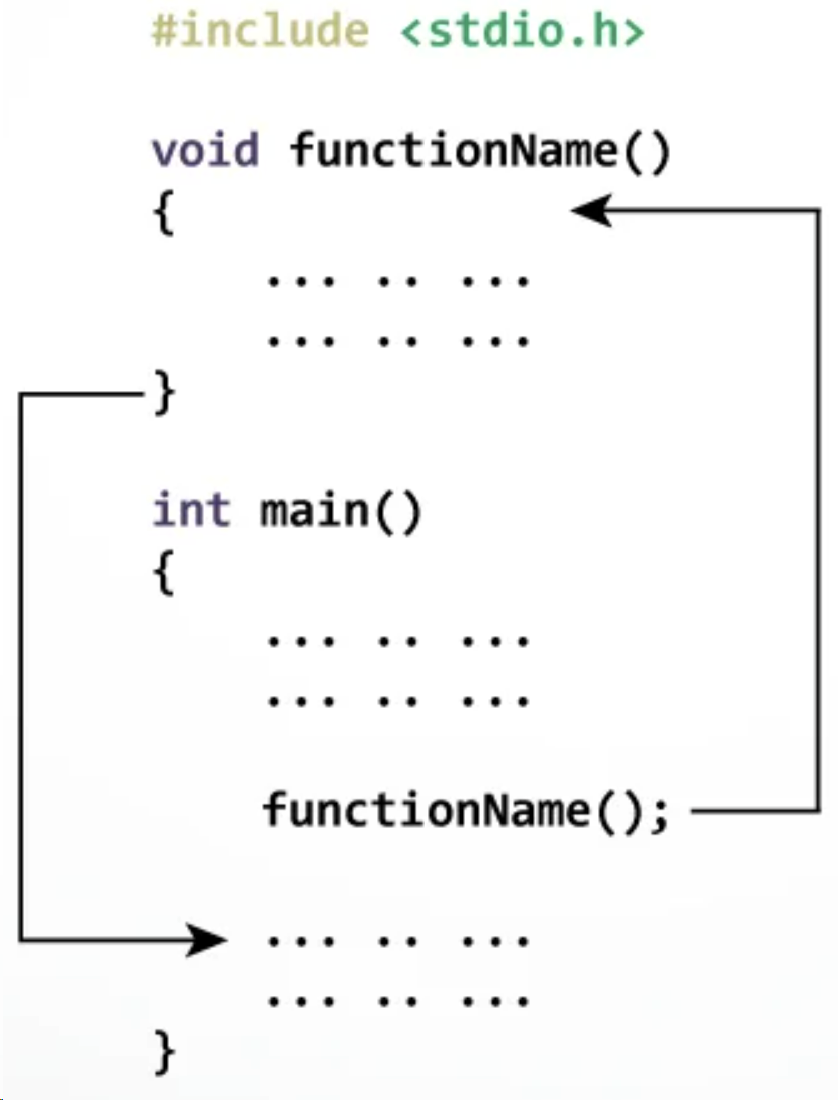
\includegraphics[width=0.45\linewidth]{P3/img/screenshot005.png}
    \caption{}
    \label{fig:memanggilfungsi}
\end{figure}

\begin{lstlisting}[language=c]
	#include <stdio.h>
  // Declaring a function to calculate a Triangle Area called TriangleArea  
% // Mendeklarasikan fungsi luasSegitiga
  // The parameters are the  value of Base and Height
% // Parameter input Alas , dan Tinggi
  // The output data type is float+
% // Output float
float TriangleArea(float Base, float Height)
{
	float Area;
	Area = 0.5*Base*Height;
	return Area;
}
int main()
{
	float Bs = 4,Hg=10,L;
    % // Memanggil Fungsi TriangleArea
	// Calling the TriangleArea function
    L=TriangleArea(Bs,Hg);
	printf("Area = %f",L);
	return 0;
}
\end{lstlisting}
\begin{enumerate}
    \item Line 5-10: Defining the function, namely \verb|Triangle Area| with
          % \item Baris 5-10:Mendefinisikan fungsi \verb*|TriangleArea| dengan 
          \begin{itemize}
              \item Two input parameters :\\
                    % \item 2 paramater input/masukan:
                    \verb*|Base| and \verb*|Height|  with \verb*|float| data type.
                    % input \verb*|Base| dan \verb*|Height|  dengan tipe data \verb*|float|.
              \item Singular output with \verb*|float| data type.
                    % \item Output bernilai tunggal dengan tipe data \verb*|float|.
          \end{itemize}
\end{enumerate}
\subsection{Function with Arguments}
% \subsection{Fungsi dengan Argumen}

\subsection{Arguments}
% \subsubsection{Argumen}

If a function is expected to use arguments,
then the variables that acts as the parameters that receive
values from these arguments must be declared beforehand. \\
% Jika suatu fungsi diharapkan untuk menggunakan argumen, 
% maka variabel sebagai parameter yang menerima nilai dari 
% argumen tersebut harus di dedeklarasikan terlebih dahulu. \\

\begin{enumerate}
    \item  \textbf{Parameters :}
          % \item  \textbf{Parameter :}
          \begin{enumerate}
              % \item Parameter adalah variabel dalam fungsi untuk merujuk 
              % ke salah satu bagian dari data yang diberikan sebagai 
              % input ke fungsi.
              \item Parameters are the variables in a function that
                    points to a part of the data that is
                    inserted into the function.
                    % \item Data ini disebut argumen.
              \item These data are called arguments.

          \end{enumerate}

    \item \textbf{Formal Parameters:}
          % \item \textbf{Formal Parameter:}
          \begin{enumerate}
              % \item Parameter yang Ditulis dalam Definisi 
              % Fungsi Disebut "Parameter Formal".
              \item Parameters that are written within the
                    function definition is called "Formal Parameters".

                    % \item Parameter formal selalu variabel, 
                    % sedangkan parameter aktual tidak harus variabel.
              \item Formal Parameters are always a variable,
                    Actual Parameter however doesn't necessarily has
                    to be a variable.

          \end{enumerate}


    \item \textbf{Actual Parameters:}
          \begin{enumerate}

              \item Parameters that are used when calling a function
                    % \item Parameter yang Ditulis ketika memanggil fungsi.

              \item Can be a form of numbers,
                    expressions, or another function call.
                    % \item Dapat berupa angka, ekspresi, atau bahkan panggilan fungsi.
          \end{enumerate}
          \begin{figure}[H]
              \centering
              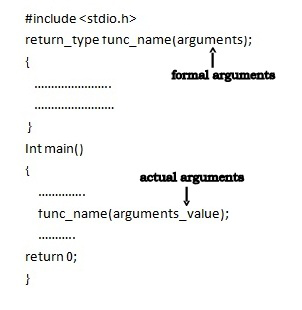
\includegraphics[width=0.5\linewidth]{P3/img/screenshot006.png}
              \caption{}
              \label{fig:parameterformalaktual}
          \end{figure}
\end{enumerate}
\subsection{Parameter Passing}
% Passing parameter merupakan aktivitas menyalurkan nilai pada 
% parameter saat memanggil fungsi. Pada umumnya, dikenal dua 
% macam passing parameter yaitu:
Parameter passing is passing a value to the parameter when calling a function.
Generally, there are two ways to pass paramaters into a function :
\begin{itemize}
    \item Pass parameter by value means to pass the
          \textbf{value} of the variable to the parameter of a function.
          % \item Pass parameter by value, yaitu menyalurkan 
          % \textbf{nilai} dari tiap parameter yang diberikan.

    \item Pass parameter by reference means to pass the
          reference of a variable \textbf{(its memory address)} to
          the paramater a function.
          % \item Pass parameter by reference, yaitu menyalurkan 
          % \textbf{alamat} dari tiap parameter yang diberikan.
\end{itemize}

\subsubsection{Passing Parameter by Value}

\begin{lstlisting}[language=c,caption = Passing by Value,label=lst:passbyvalue01]
    #include <stdio.h>

    int swapAndReturnSum(int x, int y) {
        int z;
        z = x;
        x = y;
        y = z;
        return x + y;
    }
    
    int main() {
        int a = 1;
        int b = 2;
        int sum = swapAndReturnSum(a, b);
        printf("Sum: %d\n", sum);
        printf("Value a and b now:\n");
        printf("a: %d\n", a);
        printf("b: %d\n", b);
        return 0;
    }
\end{lstlisting}

% Perhatikan potongan kode pada Listing \ref{lst:passbyvalue01}. 
% Baris 3-6 dari kode tersebut adalah operasi untuk menukar 
% nilai dari 2 variabel. Namun, apabila program tersebut 
% dijalankan, maka akan muncul output
Pay attention at the snippet above, line 3-6 of the code
in Listing \ref{lst:passbyvalue01} is a set of assignments
to swap the values of 2 variables. However, when the program
is executed, the output would be the following.
\begin{verbatim}
    sum: 3
    values a and b now:
    a: 1
    b: 2
\end{verbatim}
As you can see, the values of a and b did not swap.
When passing parameter by value, anything that is done
within the function body will have no effect on the
parameter that is "passed on" the function. The value of
the \textbf{actual parameter} will be assigned to the \textbf{formal parameter},
so we are not doing operation directly on the actual parameter.

% Nilai dari a dan b tidak bertukar. Untuk passing parameter 
% by value, apapun yang dilakukan pada function body tidak 
% akan berpengaruh pada parameter yang "dipassingkan". Nilai 
% dari parameter aktual akan diassign pada parameter formal.

\subsubsection{Passing Parameter by Reference}
% Perhatikan baris 2 pada potongan kode berikut:
Look at second line of the following code.
\begin{lstlisting}[language=c,caption = Passing by Reference,label=lst:passbyreference01]
    #include <stdio.h>

    void swap(int *x, int *y) {
        int z;
        z = *x;
        *x = *y;
        *y = z;
    }
    
    int main() {
        int a = 1;
        int b = 2;
        
        printf("Before swapping:\n");
        printf("a: %d\n", a);
        printf("b: %d\n", b);
        
        swap(&a, &b);
        
        printf("After swapping:\n");
        printf("a: %d\n", a);
        printf("b: %d\n", b);
        
        return 0;
    }
\end{lstlisting}
% Apabila program tersebut dijalankan, maka akan muncul output
The following is the ouput of the program's execution.
\begin{verbatim}
    Before swapping:
    a: 1
    b: 2
    After swapping:
    a: 2
    b: 1
\end{verbatim}

% Ketika fungsi \verb|swapAndReturnTheSum(a,b)| dipanggil, 
% alamat memori variabel a dan b "dipassingkan" pada fungsinya. 
% Sehingga pada pada potongan kode di baris 4-6, x dan y akan 
% mengacu pada memori parameter aktual yang dimasukkan di 
% baris ke 13. Ketika melakukan passing by reference, kita 
% tidak bisa memanggil fungsi dengan parameter yang tidak 
% memiliki alamat memori. Sebagai contoh 
% \verb|tukarDanKembalikansumnya(1,2)| tidak bisa dilakukan 
% karena angka 1 dan 2 bukan variabel dan tidak memiliki 
% alamat memori.
When \verb|swap(a,b)| is called,
the memory address of \verb|a| and \verb|b| is passed into
the function. Therefore, in line 4-7, the \verb|x| and
\verb|y| will point to the memory of the \textbf{actual parameter}
that is inserted in line 18, therefore we are doing assignments
directly to the actual parameter. When passing by reference,
we can't call the function with parameter that has no memory
address. As an example \verb|swapAndReturnTheSum(1,2)| cannot be
done as the number 1 and 2 doesn't have memory address.

% \subsection{Tugas Pendahuluan}
\subsection{Pre-lab Assignment}
\begin{enumerate}
    \item What is the advantages and disadvantages of function?
    \item Create a function with 2 arguments a and b of integer type that returns $a^2 + b^2$.
          % \item Masalah-masalah apa yang akan lebih mudah 
          % diselesaikan dengan menggunakan fungsi?
    \item What are the problems that can be more easily solved with functions?
\end{enumerate}

% \section{Rekursi}
\section{Recursion}
% Rekursi merujuk kepada definisi suatu hal yang dilakukan secara berulang-ulang.
Recursion refers to something that is done repeatedly
% Rekursi adalah ketika suatu fungsi dalam function bodynya memanggil fungsi itu sendiri.
Recursion in programming is when a function calls itself within its function body.
% Sebagai contoh, perhatikan potongan kode berikut:
As an example, take a look at the code below.
% \begin{lstlisting}[language=c,caption = Factorial dengan rekursi,label=lst:recursionexample01]
% int factorial(int n) 
\begin{lstlisting}[language=c,caption = Factorial with a recursion,label=lst:recursionexample01]
    int factorial(int n) {
    if (n==1)
        return 1;
    return n*factorial(n-1);
}
\end{lstlisting}
The factorial function calls another factorial function in line 4.
%Dapat dilihat bahwa fungsi factorial pada function bodynya memanggil factorial pada baris 4.
Initialy, the function $factorial(n)$ is called. This function however will return
%Pada awalnya jika fungsi $factorial(n)$ dipanggil maka dia akan mencoba untuk mengembalikan
$n\times factorial(n-1)$, then $factorial(n-1)$ will return $(n-1)\times factorial(n-1-1)$.
% $n\times factorial(n-1)$, kemudian $factorial(n-1)$ akan mengembalikan $(n-1)\times factorial(n-1-1)$.
Eventually it became like this:
% Akhirnya menjadi seperti ini:
\begin{equation*}
    \begin{split}
        factorial(n)& = n \times factorial(n-1)\\
        & = n \times (n-1) \times factorial(n-2)\\
        & = n \times (n-1) \times (n-2) \times \cdots \times 2 \times factorial(1)\\
        & = n \times (n-1) \times (n-2) \times \cdots \times 2 \times 1\\
    \end{split}
\end{equation*}

\subsection{Pre-lab Assignment}
\begin{enumerate}
    \item What are the problems that can be more easily solved with recursion?
    \item what happens if we delete the 2nd and 3rd rows in Listing \ref{lst:recursionexample01}?
    % \item Diberikan sebuah baris bilangan 1, 5, 14, 30, ... dst. Buatlah sebuah program yang mengimplementasikan fungsi rekursif untuk menentukan bilangan ke-n dari pola tersebut.
    \item Given a sequence of numbers 1, 5, 14, 30, 55, 91, ... etc. Create a program that implements a recursive function to determine the nth number in the pattern.
\end{enumerate}
% % \section{Tujuan}
\section{Goals}
\begin{itemize}[label=$\bullet$, itemsep=-1pt, leftmargin=*]
    % \item Mahasiswa mengerti tentang konsep pointer pada bahasa pemrograman C.
    \item Students are able to understand the concept of pointers in C.
          % \item Mahasiswa mengerti cara membuat dan memanggil struct pada bahasa pemrograman C.
    \item Students are able to create and call a struct in C.
          % \item Mahasiswa mengerti tentang algoritma sorting pada bahasa pemrograman C.
    \item Students are able to understand about sorting algorithm in C.
          % \item Mahasiswa mengerti tentang algoritma searching pada bahasa pemrograman C.
    \item Students are able to understand about searching algorithm in C.
          % \item Mahasiswa mampu mengaplikasikan konsep algoritma searching dan sorting pada bahasa pemrograman C.
    \item Students are able to apply the conceptof searching and sorting algorithm in C.
\end{itemize}

% \section{Pointer}
\section{Pointers}
% \subsection{Alamat Memori}
\subsection{Memory Address}
% Setiap variabel, fungsi, struct, ataupun objek lain yang dibuat dalam program mempunyai lokasi masing-masing pada memori. 
% Alokasi setiap variabel disimpan dalam alamat memori tertentu.
Every variables, functions, structs, or any object in a program have their own memory allocation.
Said Allocations are saved in certain memory addresses

% Jika  terdapat variabel \verb|var| di program Anda, \verb|&var| akan memberi alamatnya di memori.
If there are any variable \verb|var| in your program, \verb|&var| will return its address in memory
\begin{lstlisting}[language=c]
    int var = 5;
    printf("%d\n", var);
    printf("%p\n", &var);
\end{lstlisting}
\begin{center}
    % \colorbox{pink}{\parbox{0.8\linewidth}{\textbf{Catatan:} Output bisa berbeda-beda di tiap eksekusi.}}
    \colorbox{pink}{\parbox{0.8\linewidth}{\textbf{Catatan:} Output may differ in each execution.}}
\end{center}

% \subsection{Pengenalan Pointer}
\subsection{Introduction to Pinters}

% Pointer(variabel penunjuk) adalah variabel khusus yang digunakan untuk menyimpan alamat, bukan nilai.
Pointers is a special variable that serves to save addresses, not value.

% Deklarasi variabel pointer menggunakan operator \verb|*| di antara tipe data dan nama variabelnya.
To declare a pointer variable, use \verb|*| operator between the data type and it's variable name.
\begin{lstlisting}[language=c]
	#include <stdio.h>
int main()
{
	int* p; // atau
    int * p2;
	return 0;
}
\end{lstlisting}


% \subsection{Cara Kerja Pointer}
\subsection{How Pointers Work}
% Berikut adalah cara kerja dari pointer.
The following is to show how pointers work.
% \begin{lstlisting}[language=c, caption={Contoh Program Pointer}]
\begin{lstlisting}[language=c, caption={Program Example}]
    #include <stdio.h>
    int main()
    {
       int* pc, c;
       
       c = 22;
       printf("Address of c: %p\n", &c);
       printf("Value of c: %d\n\n", c);  // 22
       
       pc = &c;
       printf("Address of pointer pc: %p\n", pc);
       printf("Content of pointer pc: %d\n\n", *pc); // 22
       
       c = 11;
       printf("Address of pointer pc: %p\n", pc);
       printf("Content of pointer pc: %d\n\n", *pc); // 11
       
       *pc = 2;
       printf("Address of c: %p\n", &c);
       printf("Value of c: %d\n\n", c); // 2
       return 0;
    }
\end{lstlisting}

Explanation:\\
\begin{enumerate}
    \item \verb|int* pc, c;|
          \begin{figure}[H]
              \centering
              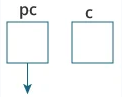
\includegraphics[width=0.2\linewidth]{P4/img/screenshot001.png}
              \caption{}
              \label{fig:satu}
          \end{figure}
    \item \verb|c = 22;|
          \begin{figure}[H]
              \centering
              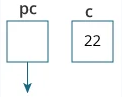
\includegraphics[width=0.2\linewidth]{P4/img/screenshot002.png}
              \caption{}
              \label{fig:dua}
          \end{figure}
    \item \verb|pc = &c;|
          \begin{figure}[H]
              \centering
              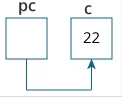
\includegraphics[width=0.2\linewidth]{P4/img/screenshot003.png}
              \caption{}
              \label{fig:tiga}
          \end{figure}
    \item \verb|c = 11;|
          \begin{figure}[H]
              \centering
              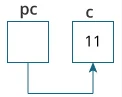
\includegraphics[width=0.2\linewidth]{P4/img/screenshot004.png}
              \caption{}
              \label{fig:empat}
          \end{figure}
    \item \verb|*pc = 2;|
          \begin{figure}[H]
              \centering
              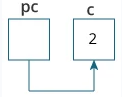
\includegraphics[width=0.2\linewidth]{P4/img/screenshot005.png}
              \caption{}
              \label{fig:lima}
          \end{figure}
\end{enumerate}

\subsection{Double Pointer}
% Variabel pointer juga dapat menunjuk variabel pointer lainnya. 
% Hal ini disebut dengan double pointer (pointer to pointer). 
% Untuk mendeklarasikan variabel double pointer, digunakan dua simbol *. 
% Kegunaan paling umum dari variabel double pointer adalah untuk membuat array dua dimensi secara dinamis.
A pointer could also point to another pointer variable. This is called a double pointer (pointer to pointer).
To declare a double pointer, we use two \verb|*| operator between the data type and its variable name.
The general usage of this double pointer variable is ti create a two dimensional array dinamically.
\begin{lstlisting}[language=c]
    int **dbPtr;
\end{lstlisting}
Variabel dbPtr di atas menyimpan alamat memori dari variabel pointer lainnya. \\
Berikut contohnya

The variable dbPtr above contains a memory address of another pointer variable.\\
Take a look at the example below.
% \begin{lstlisting}[language=c,  caption={Contoh Double Pointer}]
\begin{lstlisting}[language=c,  caption={Double Pointer Example}]
#include <stdio.h>

int main(void)
{
    int var = 23;
    int *ptr = &var;
    int **dbPtr = &ptr;

    printf("%d\n", **dbPtr);
        
    return 0;
}
\end{lstlisting}

% \subsection{Tugas Pendahuluan}
\subsection{Pre-lab Assignment}
\begin{enumerate}
    %    \item Bagaimana cara mendeklarasikan pointer ke array multidimensi?
    \item Explain how to declare a pointer to a multidimensional array?
          %    \item Buatlah program dalam bahasa C atau C++ yang mengimplementasikan 
          %    fungsi void printMatrix(int **matrix, int rows, int cols) untuk mencetak matriks 2D menggunakan pointer ke pointer. 
          %    Lalu, dalam fungsi main, buatlah matriks 2D dan panggil fungsi printMatrix untuk mencetak matriks tersebut.
    \item Create a program in C or C++ that implements void printMatrix(int **matrix, int rows, int cols) function
          to print out a 2D matrix using pointer to pointer. And then in the main function, create a 2D matrix and call the
          printMatrix function to print said matrix.
\end{enumerate}

\section{Struct}
% Dalam pemrograman C, struct (atau struktur) adalah kumpulan variabel (bisa dari tipe berbeda) di bawah satu nama. 
% Tidak seperti array yang hanya dapat menyimpan elemen dengan tipe data sama, 
% struct dapat mengelompokkan elemen dengan tipe data yang berbeda-beda.
In C, struct is a collection of variables (could be in various types) under one name. Unlike an array that could only
store elements with the same data type, struct is able to group elements with different data types.

% \subsection{Deklarasi Struct}
\subsection{Deklarasi Struct}
% Seperti variabel, struct harus dideklarasikan terlebih dahulu sebelum bisa digunakan. Pendeklarasian struct menggunakan sintaks 
% sebagai berikut.
Similar to variables, a struct must be declare first before use. Below is an example on how to declare a struct.

% \begin{lstlisting}[language=c]
% struct <nama_struct> {
%     <tipe_data_member> <nama_member>;
%     <tipe_data_member> <nama_member>;
%     <tipe_data_member> <nama_member>;
%     .
%     .
%     .
% };
% \end{lstlisting}
\begin{lstlisting}[language=c]
    struct <struct_name> {
        <member_dataType> <member_name>;
        <member_dataType> <member_name>;
        <member_dataType> <member_name>;
        .
        .
        .
    };
    \end{lstlisting}

Berikut adalah contoh deklarasi struct berdasarkan kasus Mahasiswa.
Below is a case example of struct declaration about students data.
% \begin{lstlisting}[language=c]
% struct Mahasiswa
% {
%     char *name;
%     char *address;
%     int age;
% };
% \end{lstlisting}
\begin{lstlisting}[language=c]
    struct Students
    {
        char *name;
        char *address;
        int age;
    };
    \end{lstlisting}
% \begin{center}
% 	\colorbox{pink}{\parbox{0.8\linewidth}{\textbf{Catatan:}  Menggunakan pointer * untuk data string}}
% \end{center}
\begin{center}
    \colorbox{pink}{\parbox{0.8\linewidth}{\textbf{Note:}  Use pointer * for string data type}}
\end{center}

% Setelah dideklarasikan, sebuah struct akan menjadi tipe data baru. 
% Maka dalam kasus ini, struct Mahasiswa di sini menjadi tipe data baru dengan member-member berupa \verb|nama|, 
% \verb|address|, dan \verb|age|. Untuk membuat variabel dengan tipe data struct, dilakukan dengan sintaks berikut.
After declaration, a struct will be its own data type. In this case, \textbf{Students} data type will be its own new data type
with members such as \verb|name|, \verb|address|, dan \verb|age|. Take a look at an example below to declare a variable
with the struct data type.

% \begin{lstlisting}[language=c]
%     struct <nama_struct> <nama_variabel>;
% \end{lstlisting}
\begin{lstlisting}[language=c]
    struct <struct_name> <variable_name>;
\end{lstlisting}

Example:
% \begin{lstlisting}[language=c]
%     struct Mahasiswa mhs1;
%     struct Mahasiswa mhs2;
% \end{lstlisting}
\begin{lstlisting}[language=c]
    struct Students mhs1;
    struct Students mhs2;
\end{lstlisting}
Contoh di atas menunjukkan terdapat dua variabel \verb|mhs1| dan \verb|mhs2 |bertipe struct \verb|Mahasiswa|.
The example above shows that there are two variables \verb|mhs1| and \verb|mhs2 with \verb|Mahasiswa| struct data type.

% \subsection{Akses Member Struct}
\subsection{Struct Member Access}
Bagaimana cara untuk mengakses member dari variabel struct yang telah dibuat? \\
Untuk mengakses member-member dari struct, digunakan operator dot (.) setelah nama variabelnya.
How do you access members from a struct variable? \\
To access members from a struct, we use a dot (.) operator after its variable name.

% \begin{lstlisting}[language=c]
%     <nama_variabel>.<member_struct>
% \end{lstlisting}
\begin{lstlisting}[language=c]
    <variable_name>.<member_name>
\end{lstlisting}

Example:
\begin{lstlisting}[language=c]
    mhs1.age = 69;
    mhs1.nama = Surya;
    
    mhs2.nama = Pebrianto;
    mhs2.age = 42;
\end{lstlisting}

\subsection{Pre-lab Assignment}
\begin{enumerate}
    % \item Buatlah sebuah struct yang merepresentasikan informasi tentang seorang mahasiswa, yang memiliki nama, nim, dan nilai IPK. 
    % Kemudian, buatlah program untuk menginput data mahasiswa, menampilkan data mahasiswa, dan menghitung rata-rata IPK dari 
    % sejumlah mahasiswa.
    \item Create a struct that represent informations about a students, the informations their name, student ID, and GPA.
          And then, create a program in insert student informations, display them, and calculate the average GPAs of a
          certain number of students
    \item Anda diberikan struct yang merepresentasikan titik dalam sistem koordinat dua dimensi (x, y).
          Buatlah sebuah program C untuk menghitung jarak antara dua titik yang diinputkan oleh pengguna menggunakan rumus jarak Euclidean.
    \item Create a struct that represents coordinate points in a two dimensional plane (x,y). And then create a C program to calculate
          the distance between two points that a user inputs with a Euclidean formula.
\end{enumerate}

% \section{Algoritma Sorting}
\section{Sorting algorithm}
% Sorting merupakan suatu proses penyortiran atau pengurutan sebuah data.\\
% Terdapat 2 macam pengurutan data pada sorting yaitu :
Sorting is a process of arranging or organizing data.\\
There are two types of data sorting, namely :
% \begin{enumerate}
%     \item Berdasarkan ascending (kecil ke besar).
%     \item Berdasarkan Descending (besar ke kecil).
% \end{enumerate}
\begin{enumerate}
    \item Ascending (small to large).
    \item Descending (large to small).
\end{enumerate}

\subsection{Bubble Sort}
% Bubble sort merupakan algoritma pengurutan yang membandingkan dua data yang berdekatan dan menukarnya sampai tidak dalam urutan 
% yang diinginkan. Bubble sort menggunakan teknik iterasi. Iterasi merupakan proses melakukan perulangan sebanyak data yang diketahui.
% Intinya pada iterasi melakukan perbandingan antara dua data.
Bubble sort is a sorting algorithm that compares two adjacent data points and swaps them until they are in the desired order.
Bubble sort utilizes iteration method. iteration is a process of repeating a loop as many times as there is known data.
Essentially, during each iteration, a comparison is made between two data points.

\begin{figure}[H]
    \centering
    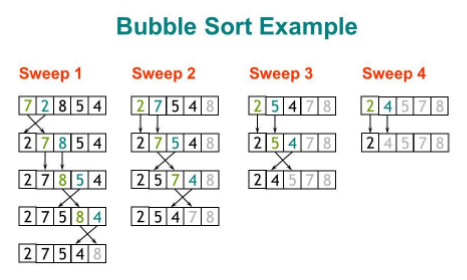
\includegraphics[width=0.7\linewidth]{P4/img/screenshot006.png}
    \caption{}
    \label{fig:enam}
\end{figure}
% \begin{lstlisting}[language=c,caption=Implementasi Bubble Sort]
\begin{lstlisting}[language=c,caption=Bubble Sort Implementation]
void swap ( int * xp , int * yp ) {
   int temp = *xp;
   *xp = *yp;
   *yp = temp;
}

void bubbleSort(int arr[], int n) {
   int i, j, swapped;        // optimized with bool `swapped`:
   for (i = 0; i < n-1; i++) {
      swapped = 0;
      for (j = 0; j < n-i-1; j++) {
         if (arr[j] > arr[j+1]) {
            swap(&arr[j], &arr[j+1]);
            swapped = 1;
         }
      }
      if (swapped == 0)
         break;
   }
}
\end{lstlisting}

\subsection{Insertion Sort}
% Insertion sort merupakan teknik sorting dengan cara menyisipkan atau memasukan setiap elemen secara berulang berulang.
% Konsep insertion sort bisa diibaratkan sebuah kartu.
Insertion sort is a sorting technique that involves repeatedly inserting or placing each element. Imagine reshuffling a
deck of cards to organize it.
\begin{figure}[H]
    \centering
    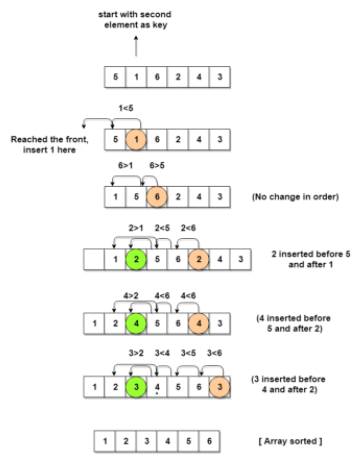
\includegraphics[width=0.5\linewidth]{P4/img/screenshot007.png}
    \caption{}
    \label{fig:tujuh}
\end{figure}
% \begin{lstlisting}[language=c,caption=Implementasi Insertion Sort],
\begin{lstlisting}[language=c,caption=Insertion Sort Implementation], 
void insertionSort(int arr[]. int n) {
   int i, key, j;
   for (i = 1; i < n; i++) {
      key = arr[i];
      j = i-1;
    
      while (j >= 0 && arr[j] > key) {
         arr[j+1] = arr[j];
         j = j-1;
      }
      arr[j+1] = key;
   }
}
\end{lstlisting}

\begin{center}
    % \colorbox{pink}{\parbox{0.8\linewidth}{\textbf{Catatan:} Terdapat berbagai algoritma sorting lain. Pelajari secara mandiri}}
    \colorbox{pink}{\parbox{0.8\linewidth}{\textbf{Note:} There are other sorting algorithms. Look it up individually}}
\end{center}

% \subsection{Tugas Pendahuluan}
\subsection{Pre-lab Assignment}
\begin{enumerate}
    % \item Urutkan array berikut menggunakan algoritma Bubble Sort:

    % Array: [5, 2, 9, 1, 5, 6]
    \item What is Big O notation?
    \item Sort the following array using Bubble Sort:

          Array: [5, 2, 9, 1, 5, 6]
    \item Hitung kompleksitas waktu (Big O) dari algoritma Insertion Sort saat mengurutkan sebuah array dengan panjang n,
          dan jelaskan bagaimana kompleksitas ini dihitung.
    \item Calculate the time complexity (Big O) of the Insertion Sort algorithm when soring an array of length n, and
          explain how this complexity is calculated
\end{enumerate}

% \section{Algoritma Searching}
\section{Searching Algorithm}
% Searching merupakan proses pencarian sebuah data yang diinginkan.
Searching is a process of looking the desired data.

\subsection{Linear Search}
Linear Search bekerja dengan melakukan pengecekan kepada semua elemen yang ada.\\
Secara garis besar, cara kerja Linear Search adalah:

Linear Search works by checking all of the existing elements.\\
Essentially, the working principle of Linear Search is:

% \begin{enumerate}
%     \item Memeriksa item satu per satu.
%     \item Apabila ditemukan, maka “ketemu”.
%     \item Jika sampai akhir belum ditemukan, maka item yang dicari tidak ada.
% \end{enumerate}
\begin{enumerate}
    \item Checking items one by one.
    \item When it is found, the program will execute any statements that needs a condition of an item to be found.
    \item If the algorithm had checked every single data, then the desired item does not exist.
\end{enumerate}

% \begin{lstlisting}[language=c,caption=Implementasi Linear Search], 
\begin{lstlisting}[language=c,caption=Linear Search Implementation], 
int linearSearch(int arr[], int n, int item) {
    int i;
    for(i = 0; i < n; ++i) {
        if(item == arr[i])
          return 1;
    }
    return -1;
}
\end{lstlisting}

\subsection{Binary Search}
% Binary Search adalah teknik pencarian di mana untuk setiap iterasinya kita membagi space pencarian menjadi hanya setengah 
% dari space pencarian awal hingga kita menemukan yang kita cari.
Binary Search is a searching technique where in each iteration we separate the searching space to half the initial searching space
until we find the desired item.

% \begin{lstlisting}[language=c,caption=Implementasi Binary Search],
\begin{lstlisting}[language=c,caption=Binary Search Implementation],   
bool f(int k, int a, int b, int n) {
   return ((k/a) * (b/a) >= n);
}

int binser(int a, int b, int n) {
   int l = 1;
   int r = 100000;
   while (r - l > 1) {
      int mid = (l + r) >> 1;
      bool can = f(mid);
      if(can)
         r = mid;
      else
         l = mid + 1;
   }
   if (can(l))
      return l;
   else
      return r;
}
\end{lstlisting}

\begin{center}
    % \colorbox{pink}{\parbox{0.8\linewidth}{\textbf{Catatan:} Terdapat berbagai algoritma searching lain. Pelajari secara mandiri}}
    \colorbox{pink}{\parbox{0.8\linewidth}{\textbf{Note:} There are other sorting algorithms. Look it up individually}}
\end{center}

% \subsection{Tugas Pendahuluan}
\subsection{Pre-lab Assignment}
\begin{enumerate}
    % \item Anda memiliki daftar nama berikut: ["Alice", "Bob", "Charlie", "David", "Eve", "Frank"]. 
    % Gunakan algoritma binary search untuk mencari apakah nama "Eve" ada dalam daftar ini. 
    % Jika ya, berapa langkah yang dibutuhkan?
    \item There is data as follows: [49, 60, 69, 42, 1, 97, 65, 77, 100, 28, 46]. Use the binary search algorithm to find out whether there are prime numbers in the data!
    \item Explain the difference between Linear Search (Sequential Search) and Binary Search.
          in what scenario that you choose one method over the other?
\end{enumerate}

\end{document}